\section{Autómata celular (Regla de life y difusión)}
Los autómatas celulares(AC) surgen en la década de 1940 con John Von Neumann, que intentaba modelar una máquina que fuera capaz de auto-replicarse, llegando así a un modelo matemático de dicha maquina con reglas complicadas sobre una red rectangular. Inicialmente fueron interpretados como conjunto de células que crecían, se reproducían y morían a medida que pasaba el tiempo. A esta similitud con el crecimiento de las células se le debe su nombre.\cite{PAGINA}

Un autómata celular se caracteriza por contar con los siguientes elementos:
\begin{enumerate}
 \item Arreglo regular. Ya sea un plano de dos dimensiones o un espacio n-dimensional, este es el espacio de evoluciones, y cada división homogénea del arreglo es llamada célula.
 \item Conjunto de estados. Es finito y cada elemento o célula del arreglo toma un valor de este conjunto de estados. También se denomina alfabeto. Puede ser expresado en valores o colores.
 \item configuración inicial. Consiste en asignar un estado a cada una de las células del espacio de evolución inicial del sistema.
 \item Vecindades. Define el conjunto contiguo de células y posición relativa respecto a cada una de ellas. A cada vecindad diferente corresponde un elemento del conjunto de estados.
 \item Función local. Es la regla de evolución que determina el comportamiento del A. C. Se conforma de una célula central y sus vecindades. Define como debe cambiar de estado cada célula dependiendo de los estados anteriores de sus vecindades. Puede ser una expresión algebraica o un grupo de ecuaciones.
\end{enumerate}

\subsection{Introducción}
\subsection{Práctica a realizar}
Este programa implementar la simulación de un autómata celular. Los puntos importantes a señalar son que cuenta con una interfaz gráfica para el usuario en la cual aparecen los unos (célula viva) y ceros (célula muerta) que son el principal elemento en este autómata celular y que son representados como pequeños cuadros que cambian su tamaño de acuerdo a la población que se tenga. Las características de este simulador son las siguientes:
\begin{itemize}
 \item Permitir seleccionar el tamaño de la población de la matriz de unos y ceros.
 \item Permitir seleccionar la regla que se utilizara en cada iteración de la simulación.
 \item Se podrá elegir la distribución de unos que habrá en la matriz.
 \item Se podrá cambiar los colores de los ceros y los unos de la simulación.
 \item Permitir guardar la matriz que se esta trabajando en un archivo de texto.
 \item Se mostrara el cambio de unos que hay a lo largo de cada iteración.
\end{itemize}
El objetivo que se tiene es mostrar una matriz de hasta 1000 por 1000 para poder observar un comportamiento que nos proporcione información.

Para el segundo parcial se realizo una mejora de este programa en esta versión se agrega la opción de insertar mosaicos ya definidos y de poder cargar un archivo con una configuración inicial del juego de la vida. Otra funcionalidad que faltaba en la versión anterior y que se agrego en este programa es una barra para poder moverse a lo largo de toda la sección de simulación y así poder apreciar la simulación por completo.

Los patrones que se eligieron son los más comunes que se pueden encontrar con estas dos reglas y que generan nuevos patrones a lo largo de la simulación del programa. Los mosaicos que se agregaron son algunos que se generan con la regla de life y con la regla de difusión. Las siguientes figuras son las cinco que se pueden insertar en el simulador.

\begin{figure}[H]
\begin{center}
 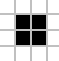
\includegraphics[width=4cm, height=4cm]{./img/cuadrado.png}
 \caption{Patrón estático que se genera con la regla 2333}
 \label{fig:cuadrado}
\end{center}
\end{figure}

\begin{figure}[H]
\begin{center}
 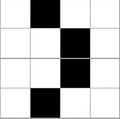
\includegraphics[width=4cm, height=4cm]{./img/glider.png}
 \caption{Glider que se genera con la regla 7722}
 \label{fig:glider}
\end{center}
\end{figure}

\begin{figure}[H]
\begin{center}
 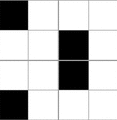
\includegraphics[width=4cm, height=4cm]{./img/glider2.png}
 \caption{Glider que se genera con la regla 7722}
 \label{fig:glider2}
\end{center}
\end{figure}

\begin{figure}[H]
\begin{center}
 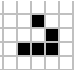
\includegraphics[width=4cm, height=4cm]{./img/glider3.png}
 \caption{Glider que se genera con la regla 2333}
 \label{fig:glider3}
\end{center}
\end{figure}

\begin{figure}[H]
\begin{center}
 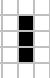
\includegraphics[width=4cm, height=5cm]{./img/oscilador.png}
 \caption{Oscilador que se genera con la regla 2333}
 \label{fig:oscilador}
\end{center}
\end{figure}

\subsection{Desarrollo}
Archivo: gol.py
En este archivo se encuentra la clase que controla todo el juego de la vida, desde el como se muestra en pantalla a como trabaja. El código fue desarrollado en python 3 y se utilizo la biblioteca tkinter.
\begin{lstlisting}[language=Python]
 from tkinter import Tk, Canvas, Frame, Button, Entry, Label, Scale, filedialog
from tkinter import BOTH, TOP, LEFT, HORIZONTAL, Y, RIGHT, VERTICAL, PhotoImage
from tkinter import Scrollbar
import numpy as np
from tkcolorpicker import askcolor
import datetime
import time


dict_tipos = {
    "nada": 0,
    "cubo": 1,
    "glider": 2,
    "glider2": 3,
    "glider3": 4,
    "oscilador": 5,
}


class Ventana(Frame):
    def __init__(self, parent):
        Frame.__init__(self, parent)
        self.parent = parent

        # Elementos interfaz
        self.ceros = "white"
        self.unos = "black"
        self.regla = [2, 3, 3, 3]
        self.e1 = None
        self.e2 = None
        self.contador = 0
        self.colorBtn1 = None
        self.colorBtn2 = None
        self.barra = None
        self.canvas = None
        self.cubo_image = None
        self.glider = None
        self.glider2 = None
        self.glider3 = None
        self.oscilador = None
        # variables del juego de la vida
        self.pausa = True
        self.tam = 100
        self.tam_cuadro = 10
        self.distribucion = .5
        self.cuadritos = np.zeros(shape=(self.tam, self.tam), dtype=int)
        self.celulas = np.random.randint(2, size=(self.tam, self.tam), dtype=int)
        self.tiempo = 0
        self.tipo_insertar = dict_tipos["nada"]
        # Historial de unos
        self.nom_archivo = None

    def iniciar(self):
        self.nom_archivo = "{}.csv".format(self.obtener_hora())
        archivo = open(self.nom_archivo, "w")
        archivo.close()
        self.canvas.delete('all')
        self.update_idletasks()
        self.pausa = True
        self.contador = 0
        self.tiempo = 0
        self.tam = int(self.e2.get())
        self.tam_cuadro = 0
        while self.tam_cuadro*self.tam < 1000:
            self.tam_cuadro += 1
        if self.tam_cuadro*self.tam > 1000:
            self.tam_cuadro -= 1
        self.distribucion = self.barra.get()/100
        self.celulas = np.random.choice([1, 0], size=(self.tam, self.tam), p=[self.distribucion, 1-self.distribucion])
        self.cuadritos = np.zeros(shape=(self.tam, self.tam), dtype=int)
        texto = self.e1.get().split(",")
        self.regla[0] = int(texto[0])
        self.regla[1] = int(texto[1])
        self.regla[2] = int(texto[2])
        self.regla[3] = int(texto[3])
        self.contar_unos()
        print(self.contador)
        self.re_dibujar()

    def contar_unos(self):
        for i in range(self.tam):
            for j in range(self.tam):
                if self.celulas[i, j] == 1:
                    self.contador += 1

        print("contador_unos : {}".format(self.contador))

    def pulsar_cuadrito(self, event):
        item = self.canvas.find_closest(event.x, event.y)[0]
        i, j = np.where(self.cuadritos == item)
        print("{}, {}".format(i[0], j[0]))
        if self.tipo_insertar == dict_tipos["nada"]:
            if self.canvas.itemcget(item, "fill") == self.unos:
                self.canvas.itemconfig(item, fill=self.ceros)
                self.celulas[i[0]][j[0]] = 0
                self.contador -= 1
            else:
                self.canvas.itemconfig(item, fill=self.unos)
                self.celulas[i[0]][j[0]] = 1
                self.contador += 1
        elif self.tipo_insertar == dict_tipos["cubo"]:
            print("cubo")
            print(self.celulas)
            self.insertar_cubo(i[0], j[0])
            print(self.celulas)
        elif self.tipo_insertar == dict_tipos["glider"]:
            print("glider")
            self.insertar_glider(i[0], j[0])
        elif self.tipo_insertar == dict_tipos["glider2"]:
            print("glider2")
            self.insertar_glider_dos(i[0], j[0])
        elif self.tipo_insertar == dict_tipos["glider3"]:
            print("glider3")
            self.insertar_glider_tres(i[0], j[0])
        elif self.tipo_insertar == dict_tipos["oscilador"]:
            print("oscilador")
            self.insertar_oscilador(i[0], j[0])

        self.tipo_insertar = dict_tipos["nada"]

    def insertar_cubo(self, x1, y1):
        x2 = x1 + 1
        y2 = y1 + 1
        item1 = self.cuadritos[x1, y1]
        item2 = self.cuadritos[x1, y2]
        item3 = self.cuadritos[x2, y1]
        item4 = self.cuadritos[x2, y2]

        if self.celulas[x1, y1] == 0:
            self.celulas[x1, y1] = 1
            self.contador += 1
            self.canvas.itemconfig(item1, fill=self.unos)
        if self.celulas[x1, y2] == 0:
            self.celulas[x1, y2] = 1
            self.contador += 1
            self.canvas.itemconfig(item2, fill=self.unos)
        if self.celulas[x2, y1] == 0:
            self.celulas[x2, y1] = 1
            self.contador += 1
            self.canvas.itemconfig(item3, fill=self.unos)
        if self.celulas[x2, y2] == 0:
            self.celulas[x2, y2] = 1
            self.contador += 1
            self.canvas.itemconfig(item4, fill=self.unos)

    def insertar_oscilador(self, i1, j1):
        i0 = i1 - 1
        i2 = i1 + 1
        item0 = self.cuadritos[i0, j1]
        item1 = self.cuadritos[i1, j1]
        item2 = self.cuadritos[i2, j1]

        if self.celulas[i0, j1] == 0:
            self.celulas[i0, j1] = 1
            self.contador += 1
            self.canvas.itemconfig(item0, fill=self.unos)

        if self.celulas[i1, j1] == 0:
            self.celulas[i1, j1] = 1
            self.contador += 1
            self.canvas.itemconfig(item1, fill=self.unos)

        if self.celulas[i2, j1] == 0:
            self.celulas[i2, j1] = 1
            self.contador += 1
            self.canvas.itemconfig(item2, fill=self.unos)

    def insertar_glider(self, i1, j1):
        j2 = j1 + 1
        i2 = i1 + 1
        i3 = i2 + 1
        i4 = i3 + 1

        item1 = self.cuadritos[i1, j1]
        item2 = self.cuadritos[i1, j2]
        item3 = self.cuadritos[i2, j1]
        item4 = self.cuadritos[i2, j2]
        item5 = self.cuadritos[i3, j1]
        item6 = self.cuadritos[i3, j2]
        item7 = self.cuadritos[i4, j1]
        item8 = self.cuadritos[i4, j2]

        if self.celulas[i1, j1] == 0:
            self.celulas[i1, j1] = 1
            self.contador += 1
            self.canvas.itemconfig(item1, fill=self.unos)
        if self.celulas[i1, j2] == 1:
            self.celulas[i1, j2] = 0
            self.contador -= 1
            self.canvas.itemconfig(item2, fill=self.ceros)

        if self.celulas[i2, j1] == 1:
            self.celulas[i2, j1] = 0
            self.contador -= 1
            self.canvas.itemconfig(item3, fill=self.ceros)
        if self.celulas[i2, j2] == 0:
            self.celulas[i2, j2] = 1
            self.contador += 1
            self.canvas.itemconfig(item4, fill=self.unos)

        if self.celulas[i3, j1] == 1:
            self.celulas[i3, j1] = 0
            self.contador -= 1
            self.canvas.itemconfig(item5, fill=self.ceros)
        if self.celulas[i3, j2] == 0:
            self.celulas[i3, j2] = 1
            self.contador += 1
            self.canvas.itemconfig(item6, fill=self.unos)

        if self.celulas[i4, j1] == 0:
            self.celulas[i4, j1] = 1
            self.contador += 1
            self.canvas.itemconfig(item7, fill=self.unos)
        if self.celulas[i1, j2] == 1:
            self.celulas[i1, j2] = 0
            self.contador -= 1
            self.canvas.itemconfig(item8, fill=self.ceros)

    def insertar_glider_dos(self, i1, j1):
        i2 = i1 + 1
        i3 = i2 + 1
        i4 = i3 + 1
        j2 = j1 + 1
        j3 = j2 + 1

        item1 = self.cuadritos[i1, j1]
        item2 = self.cuadritos[i1, j2]
        item3 = self.cuadritos[i1, j3]
        item4 = self.cuadritos[i2, j1]
        item5 = self.cuadritos[i2, j2]
        item6 = self.cuadritos[i2, j3]
        item7 = self.cuadritos[i3, j1]
        item8 = self.cuadritos[i3, j2]
        item9 = self.cuadritos[i3, j3]
        item10 = self.cuadritos[i4, j1]
        item11 = self.cuadritos[i4, j2]
        item12 = self.cuadritos[i4, j3]

        if self.celulas[i1, j1] == 0:
            self.celulas[i1, j1] = 1
            self.contador += 1
            self.canvas.itemconfig(item1, fill=self.unos)
        if self.celulas[i1, j2] == 1:
            self.celulas[i1, j2] = 0
            self.contador -= 1
            self.canvas.itemconfig(item2, fill=self.ceros)
        if self.celulas[i1, j3] == 1:
            self.celulas[i1, j2] = 0
            self.contador -= 1
            self.canvas.itemconfig(item3, fill=self.ceros)

        if self.celulas[i2, j1] == 1:
            self.celulas[i2, j1] = 0
            self.contador -= 1
            self.canvas.itemconfig(item4, fill=self.ceros)
        if self.celulas[i2, j2] == 1:
            self.celulas[i2, j2] = 0
            self.contador -= 1
            self.canvas.itemconfig(item5, fill=self.ceros)
        if self.celulas[i2, j3] == 0:
            self.celulas[i2, j3] = 1
            self.contador += 1
            self.canvas.itemconfig(item6, fill=self.unos)

        if self.celulas[i3, j1] == 1:
            self.celulas[i3, j1] = 0
            self.contador -= 1
            self.canvas.itemconfig(item7, fill=self.ceros)
        if self.celulas[i3, j2] == 1:
            self.celulas[i3, j2] = 0
            self.contador -= 1
            self.canvas.itemconfig(item8, fill=self.ceros)
        if self.celulas[i3, j3] == 0:
            self.celulas[i3, j3] = 1
            self.contador += 1
            self.canvas.itemconfig(item9, fill=self.unos)

        if self.celulas[i4, j1] == 0:
            self.celulas[i4, j1] = 1
            self.contador += 1
            self.canvas.itemconfig(item10, fill=self.unos)
        if self.celulas[i4, j2] == 1:
            self.celulas[i4, j2] = 0
            self.contador -= 1
            self.canvas.itemconfig(item11, fill=self.ceros)
        if self.celulas[i4, j3] == 1:
            self.celulas[i4, j3] = 0
            self.contador -= 1
            self.canvas.itemconfig(item12, fill=self.ceros)

    def insertar_glider_tres(self, i2, j2):
        i1 = i2 - 1
        i3 = i2 + 1
        j1 = j2 - 1
        j3 = j2 + 1

        item1 = self.cuadritos[i1, j1]
        item2 = self.cuadritos[i1, j2]
        item3 = self.cuadritos[i1, j3]
        item4 = self.cuadritos[i2, j1]
        item5 = self.cuadritos[i2, j2]
        item6 = self.cuadritos[i2, j3]
        item7 = self.cuadritos[i3, j1]
        item8 = self.cuadritos[i3, j2]
        item9 = self.cuadritos[i3, j3]

        if self.celulas[i1, j1] == 1:
            self.celulas[i1, j1] = 0
            self.contador -= 1
            self.canvas.itemconfig(item1, fill=self.ceros)
        if self.celulas[i1, j2] == 0:
            self.celulas[i1, j2] = 1
            self.contador += 1
            self.canvas.itemconfig(item2, fill=self.unos)
        if self.celulas[i1, j3] == 1:
            self.celulas[i1, j2] = 0
            self.contador -= 1
            self.canvas.itemconfig(item3, fill=self.ceros)

        if self.celulas[i2, j1] == 1:
            self.celulas[i2, j1] = 0
            self.contador -= 1
            self.canvas.itemconfig(item4, fill=self.ceros)
        if self.celulas[i2, j2] == 1:
            self.celulas[i2, j2] = 0
            self.contador -= 1
            self.canvas.itemconfig(item5, fill=self.ceros)
        if self.celulas[i2, j3] == 0:
            self.celulas[i2, j3] = 1
            self.contador += 1
            self.canvas.itemconfig(item6, fill=self.unos)

        if self.celulas[i3, j1] == 0:
            self.celulas[i3, j1] = 1
            self.contador += 1
            self.canvas.itemconfig(item7, fill=self.unos)
        if self.celulas[i3, j2] == 0:
            self.celulas[i3, j2] = 1
            self.contador += 1
            self.canvas.itemconfig(item8, fill=self.unos)
        if self.celulas[i3, j3] == 0:
            self.celulas[i3, j3] = 1
            self.contador += 1
            self.canvas.itemconfig(item9, fill=self.unos)

    def re_dibujar(self):
        print("REDIBUJAR")
        for i in range(self.tam):
            for j in range(self.tam):
                if self.celulas[i, j] == 0:
                    self.cuadritos[i, j] = self.canvas.create_rectangle(0 + (j * self.tam_cuadro),
                                                                        0 + (i * self.tam_cuadro),
                                                                        self.tam_cuadro + (j * self.tam_cuadro),
                                                                        self.tam_cuadro + (i * self.tam_cuadro),
                                                                        fill=self.ceros, width=0, tag="btncuadrito")
                else:
                    self.cuadritos[i, j] = self.canvas.create_rectangle(0 + (j * self.tam_cuadro),
                                                                        0 + (i * self.tam_cuadro),
                                                                        self.tam_cuadro + (j * self.tam_cuadro),
                                                                        self.tam_cuadro + (i * self.tam_cuadro),
                                                                        fill=self.unos, width=0, tag="btncuadrito")

        self.canvas.tag_bind("btncuadrito", "<Button-1>", self.pulsar_cuadrito)
        self.update_idletasks()

    def init_ui(self):
        self.parent.title("Juego de la vida")
        self.pack(fill=BOTH, expand=1)

        self.canvas = Canvas(self, relief='raised', width=1000, height=1000)
        scroll = Scrollbar(self, orient=VERTICAL)
        scroll.pack(side=RIGHT, fill=Y)
        scroll.config(command=self.canvas.yview)

        self.canvas.config(yscrollcommand=scroll.set)
        self.canvas.pack(side=LEFT)


        Label(self, text="Regla:").pack(side=TOP)
        self.e1 = Entry(self, fg="black", bg="white")
        self.e1.insert(10, "2,3,3,3")
        self.e1.pack(side=TOP)

        Label(self, text="Tamanio:").pack(side=TOP)
        self.e2 = Entry(self, fg="black", bg="white")
        self.e2.insert(10, "100")
        self.e2.pack(side=TOP)

        Label(self, text="Porcentaje de unos").pack(side=TOP)
        self.barra = Scale(self, from_=0, to=100, orient=HORIZONTAL, tickinterval=50)
        self.barra.set(50)
        self.barra.pack(side=TOP)

        btn_iniciar = Button(self, text="Iniciar/Reiniciar", command=self.iniciar)
        btn_iniciar.pack(side=TOP)

        button1 = Button(self, text="Pausa/Reanudar", command=self.empezar_dentener)
        button1.pack(side=TOP)

        self.colorBtn1 = Button(self, text="Selecciona el color de unos", command=self.get_color_unos, bg=self.unos)
        self.colorBtn1.pack(side=TOP)

        self.colorBtn2 = Button(self, text="Selecciona el color de ceros", command=self.get_color_ceros, bg=self.ceros)
        self.colorBtn2.pack(side=TOP)

        btn_save = Button(self, text="Guardar", command=self.guardar)
        btn_save.pack(side=TOP)

        btn_cargar = Button(self, text="Cargar Matriz", command=self.cargar)
        btn_cargar.pack(side=TOP)

        self.cubo_image = PhotoImage(file="./data/cuadrado.png")
        btn_cubo = Button(self, image=self.cubo_image, command=self.seleccionar_cubo)
        btn_cubo.pack(side=TOP)

        self.glider = PhotoImage(file="./data/glider.png")
        self.glider = self.glider.subsample(2)
        btn_glider = Button(self, image=self.glider, command=self.seleccionar_glider)
        btn_glider.pack(side=TOP)

        self.glider2 = PhotoImage(file="./data/glider2.png")
        self.glider2 = self.glider2.subsample(2)
        btn_glider2 = Button(self, image=self.glider2, command=self.seleccionar_glider_dos)
        btn_glider2.pack(side=TOP)

        self.glider3 = PhotoImage(file="./data/glider3.png")
        btn_glider3 = Button(self, image=self.glider3, command=self.seleccionar_glider_tres)
        btn_glider3.pack(side=TOP)

        self.oscilador = PhotoImage(file="./data/oscilador.png")
        btn_osilador = Button(self, image=self.oscilador, command=self.seleccionar_oscilador)
        btn_osilador.pack(side=TOP)

    def seleccionar_glider(self):
        self.tipo_insertar = dict_tipos["glider"]

    def seleccionar_glider_dos(self):
        self.tipo_insertar = dict_tipos["glider2"]

    def seleccionar_glider_tres(self):
        self.tipo_insertar = dict_tipos["glider3"]

    def seleccionar_oscilador(self):
        self.tipo_insertar = dict_tipos["oscilador"]

    def seleccionar_cubo(self):
        self.tipo_insertar = dict_tipos["cubo"]

    @staticmethod
    def abrir_archivo():
        print("abrir archivo")
        ga = filedialog.askopenfilename(title="Selecciona un archivo",
                                        filetypes=(("CSV", "*.csv"), ("Archivo de texto", "*.txt"),
                                                   ("Todos los archivos", "*.*")))
        return ga

    def actualizar_color_matriz(self):
        for i in range(self.tam):
            for j in range(self.tam):
                if self.celulas[i][j] == 0:
                    self.canvas.itemconfig(self.cuadritos[i][j], fill=self.ceros)
                else:
                    self.canvas.itemconfig(self.cuadritos[i][j], fill=self.unos)

        self.update_idletasks()

    def get_color_unos(self):
        color = askcolor()
        if not color[1] is None:
            self.unos = color[1]
            self.colorBtn1.configure(bg=self.unos)
            self.actualizar_color_matriz()

    def get_color_ceros(self):
        color = askcolor()
        if not color[1] is None:
            self.ceros = color[1]
            self.colorBtn2.configure(bg=self.ceros)
            self.actualizar_color_matriz()

    def guardar(self):
        temp_nom = "respaldo-{}.csv".format(self.obtener_hora())
        archivo = open(temp_nom, 'a')
        for i in range(self.tam):
            for j in range(self.tam):
                archivo.write("{} ".format(self.celulas[i, j]))
            archivo.write("\n")

        archivo.write("\n")
        archivo.close()

    def cargar(self):
        print("Cargar archivo")
        temp_archivo = self.abrir_archivo()
        self.celulas = np.loadtxt(temp_archivo, dtype=int)
        self.canvas.delete('all')
        self.nom_archivo = "{}.csv".format(self.obtener_hora())
        archivo = open(self.nom_archivo, "w")
        archivo.close()
        texto = self.e1.get().split(",")
        self.regla[0] = int(texto[0])
        self.regla[1] = int(texto[1])
        self.regla[2] = int(texto[2])
        self.regla[3] = int(texto[3])
        self.tam = self.celulas.shape[0]
        self.cuadritos = np.zeros(shape=(self.tam, self.tam), dtype=int)
        self.tam_cuadro = 0
        self.contador = 0
        while self.tam_cuadro * self.tam < 1000:
            self.tam_cuadro += 1
        if self.tam_cuadro * self.tam > 1000:
            self.tam_cuadro -= 1
        self.contar_unos()
        self.re_dibujar()

    def empezar_dentener(self):
        print("empezar_detener")
        self.pausa = not self.pausa
        self.animacion()

    def animacion(self):
        if not self.pausa:
            archivo = open(self.nom_archivo, "a")
            archivo.write("{},{}\n".format(self.tiempo, self.contador))
            archivo.close()
            nueva_poblacion = self.celulas.copy()
            for i in range(self.tam):
                for j in range(self.tam):
                    vecinos = self.revisar_vecinos(i, j)
                    if self.celulas[i, j] == 1:
                        if vecinos < self.regla[0] or vecinos > self.regla[1]:
                            nueva_poblacion[i, j] = 0
                            self.canvas.itemconfig(self.cuadritos[i][j], fill=self.ceros)
                            self.contador -= 1
                    else:
                        if self.regla[2] <= vecinos <= self.regla[3]:
                            nueva_poblacion[i, j] = 1
                            self.canvas.itemconfig(self.cuadritos[i][j], fill=self.unos)
                            self.contador += 1

            self.celulas[:] = nueva_poblacion[:]
            self.update_idletasks()
            print("Termino el t={}".format(self.tiempo))
            self.tiempo += 1
            self.after(50, self.animacion)

    def revisar_vecinos(self, i, j):
        vecinos = self.celulas[i - 1, j - 1]
        vecinos += self.celulas[i - 1, j]
        vecinos += self.celulas[i - 1, (j + 1) % self.tam]
        vecinos += self.celulas[i, (j + 1) % self.tam]
        vecinos += self.celulas[(i + 1) % self.tam, (j + 1) % self.tam]
        vecinos += self.celulas[(i + 1) % self.tam, j]
        vecinos += self.celulas[(i + 1) % self.tam, j - 1]
        vecinos += self.celulas[i, j - 1]
        return vecinos

    @staticmethod
    def obtener_hora():
        return datetime.datetime.fromtimestamp(time.time()).strftime('%Y-%m-%d_%H:%M:%S')


# 2 2 7 7
def main():
    root = Tk()
    root.geometry('1360x750+0+0')
    app = Ventana(root)
    app.init_ui()
    app.mainloop()


main()

\end{lstlisting}

Archivo: grafica.py
En este archivo se encuentra el código que se encarga de graficar la historia de unos a lo largo de la animación, al igual que el archivo anterior se utilizo python 3, sin embargo en la graficación se realizo con la biblioteca matplotlib.
\begin{lstlisting}[language=Python]
import matplotlib.pyplot as plt
import matplotlib.animation as animation

fig = plt.figure('Historial de unos')
fig.suptitle("Historial de unos")
ax1 = fig.add_subplot(1, 1, 1)
def animacion(i):
    info = open("grafica.txt", "r").read()
    lineas = info.split("\n")
    xs = []
    ys = []

    for linea in lineas:
        if len(linea) > 1:
            x,y = linea.split(",")
            xs.append(int(x))
            ys.append(int(y))
    ax1.clear()
    ax1.plot(xs, ys)

ani = animation.FuncAnimation(fig, animacion, interval=1000)

plt.show()
\end{lstlisting}

\subsection{Pruebas}

\begin{figure}[H]
\begin{center}
 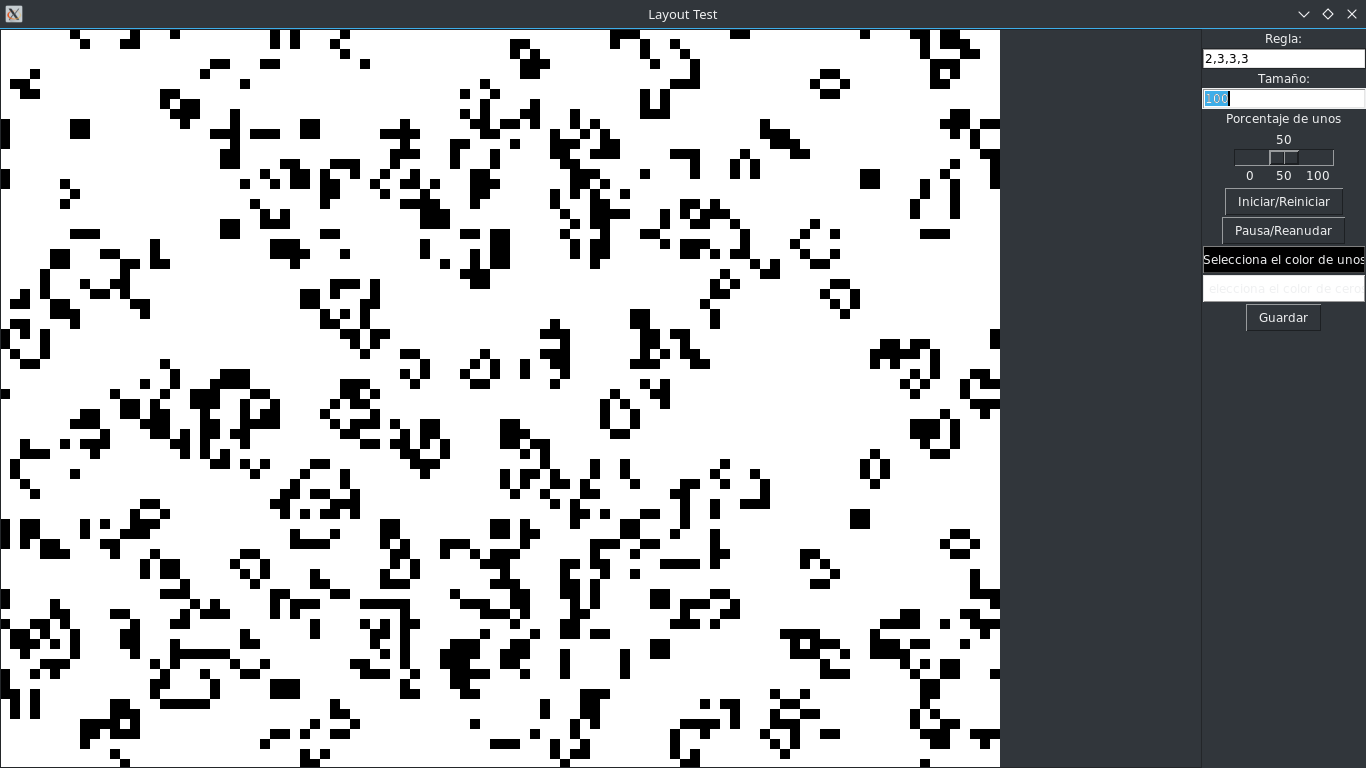
\includegraphics[width=13cm, height=6cm]{./img/gol.png}
 \caption{Juego de la vida con la regla 2333}
 \label{fig:gol}
\end{center}
\end{figure}

\begin{figure}[H]
\begin{center}
 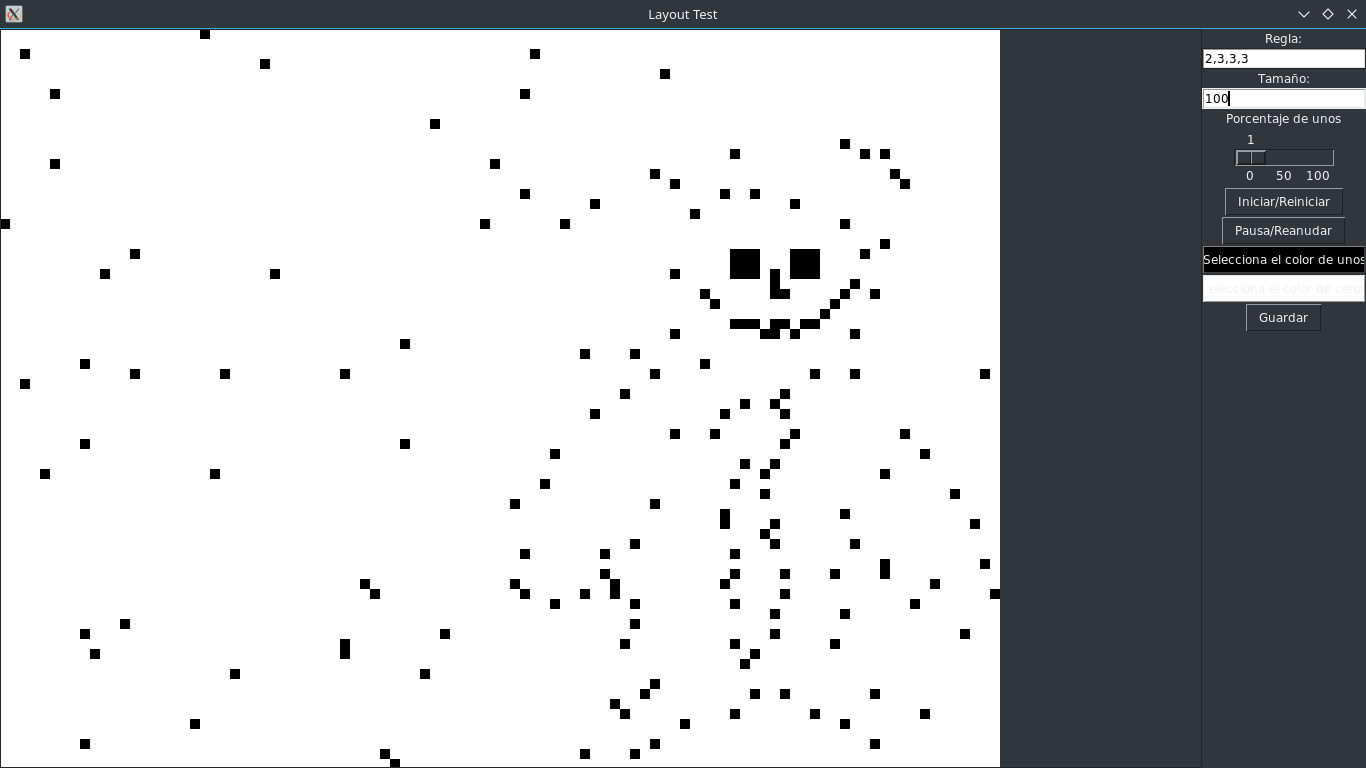
\includegraphics[width=13cm, height=6cm]{./img/gol_celulas.png}
 \caption{Juego de la vida con células seleccionadas por el usuario}
 \label{fig:gol_celulas}
\end{center}
\end{figure}

\begin{figure}[H]
\begin{center}
 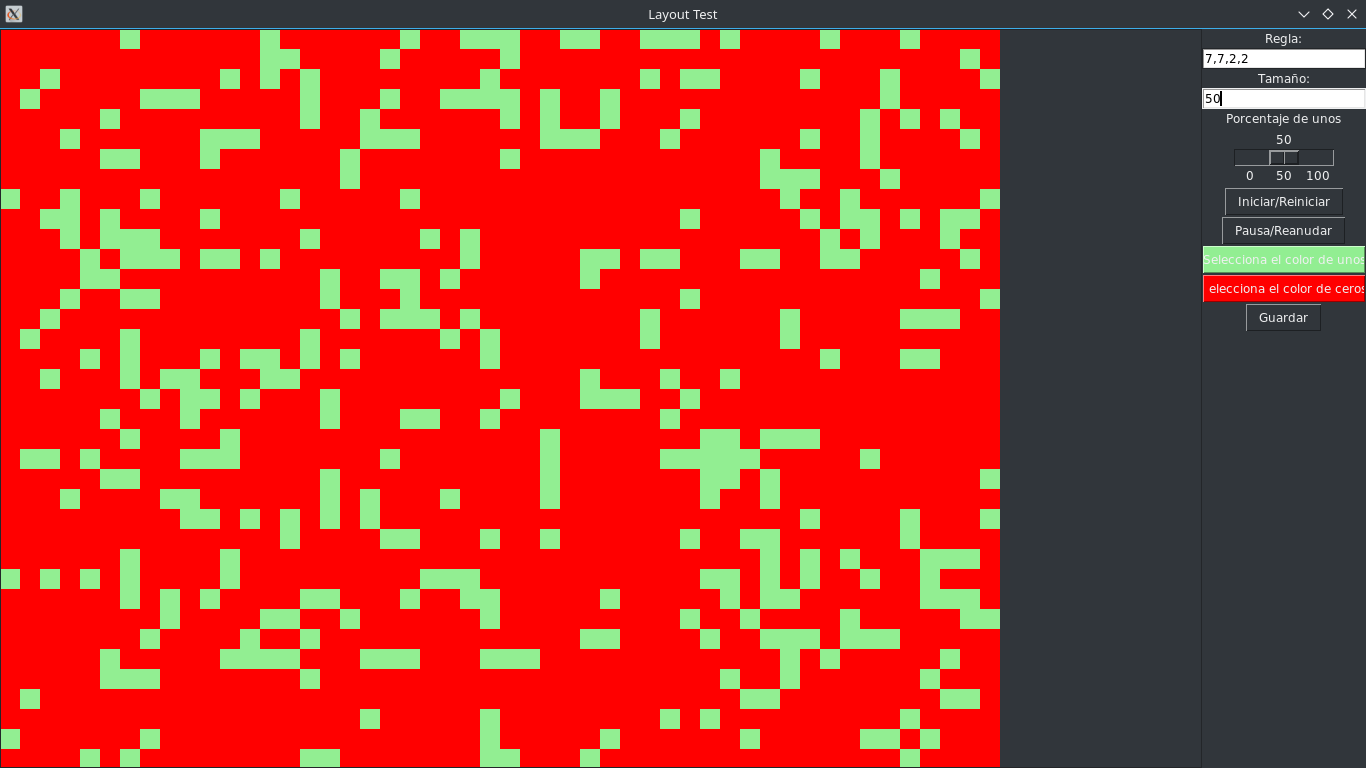
\includegraphics[width=13cm, height=6cm]{./img/gol_colores.png}
 \caption{Juego de la vida cambiando los colores y la regla 7722}
 \label{fig:gol_colores}
\end{center}
\end{figure}

\begin{figure}[H]
\begin{center}
 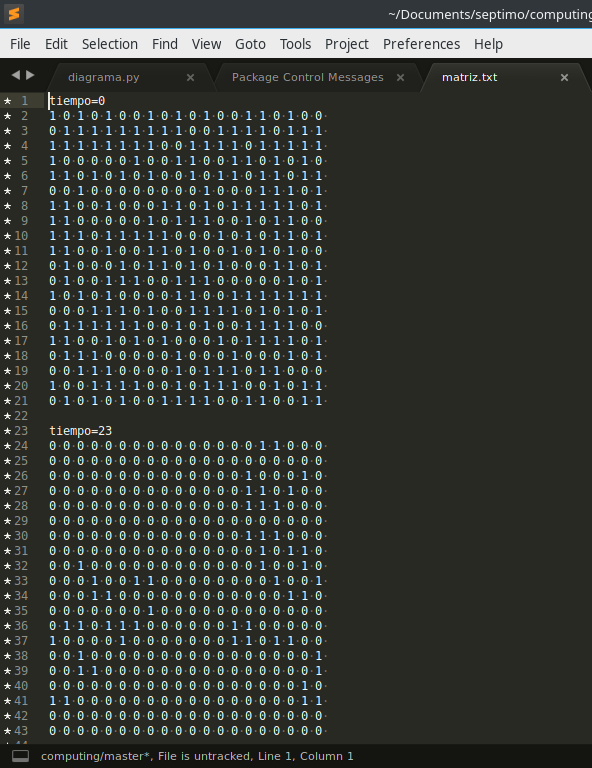
\includegraphics[width=8cm, height=13cm]{./img/matriz.png}
 \caption{Matriz que se guarda}
 \label{fig:matriz}
\end{center}
\end{figure}

\subsubsection{Análisis de poblaciones}
En esta parte se hicieron pruebas con la regla de life y difusión aumentando la densidad de la población de 10 en 10 por ciento hasta llegar al máximo de 90 por ciento debido que en un 100 por ciento no se aprecia nada al igual que en cero, las pruebas de realizaron tras 500 o 1000 generaciones en una matriz de 100 por 100.

\begin{figure}[H]
\begin{center}
 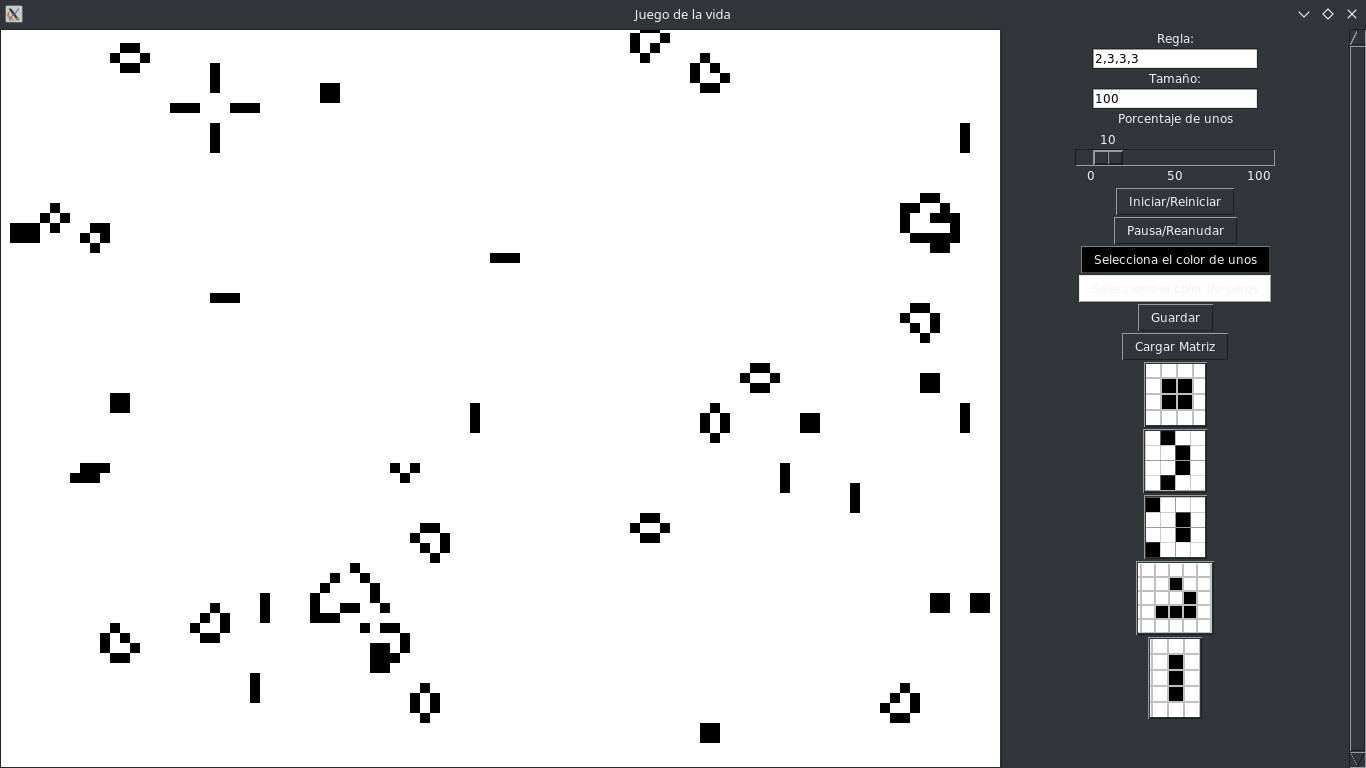
\includegraphics[width=12cm, height=8cm]{./img/life10.png}
 \caption{Regla de life con una probabilidad de unos de 10\%}
 \label{fig:life10}
\end{center}
\end{figure}

\begin{figure}[H]
\begin{center}
 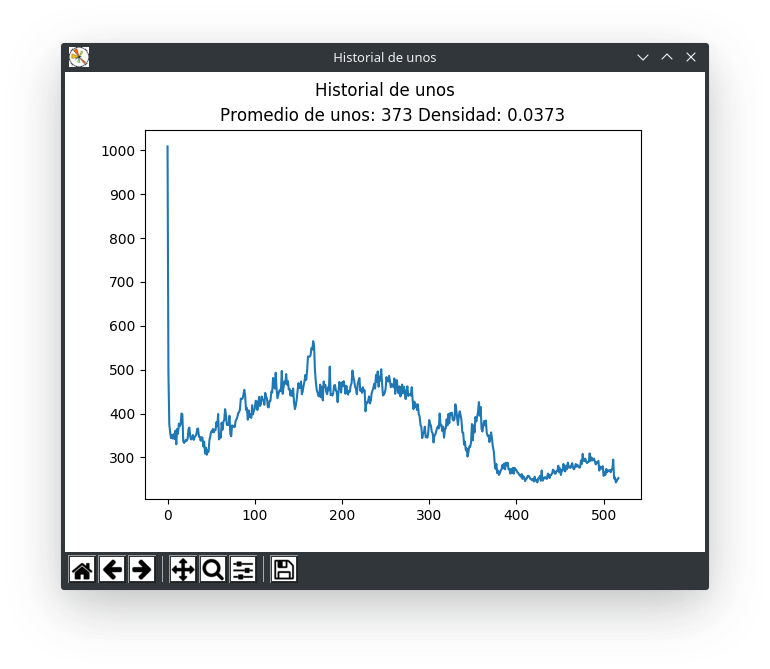
\includegraphics[width=12cm, height=8cm]{./img/life10grafica.png}
 \caption{Comportamiento de la población de la simulación anterior}
 \label{fig:life10grafica}
\end{center}
\end{figure}

\begin{figure}[H]
\begin{center}
 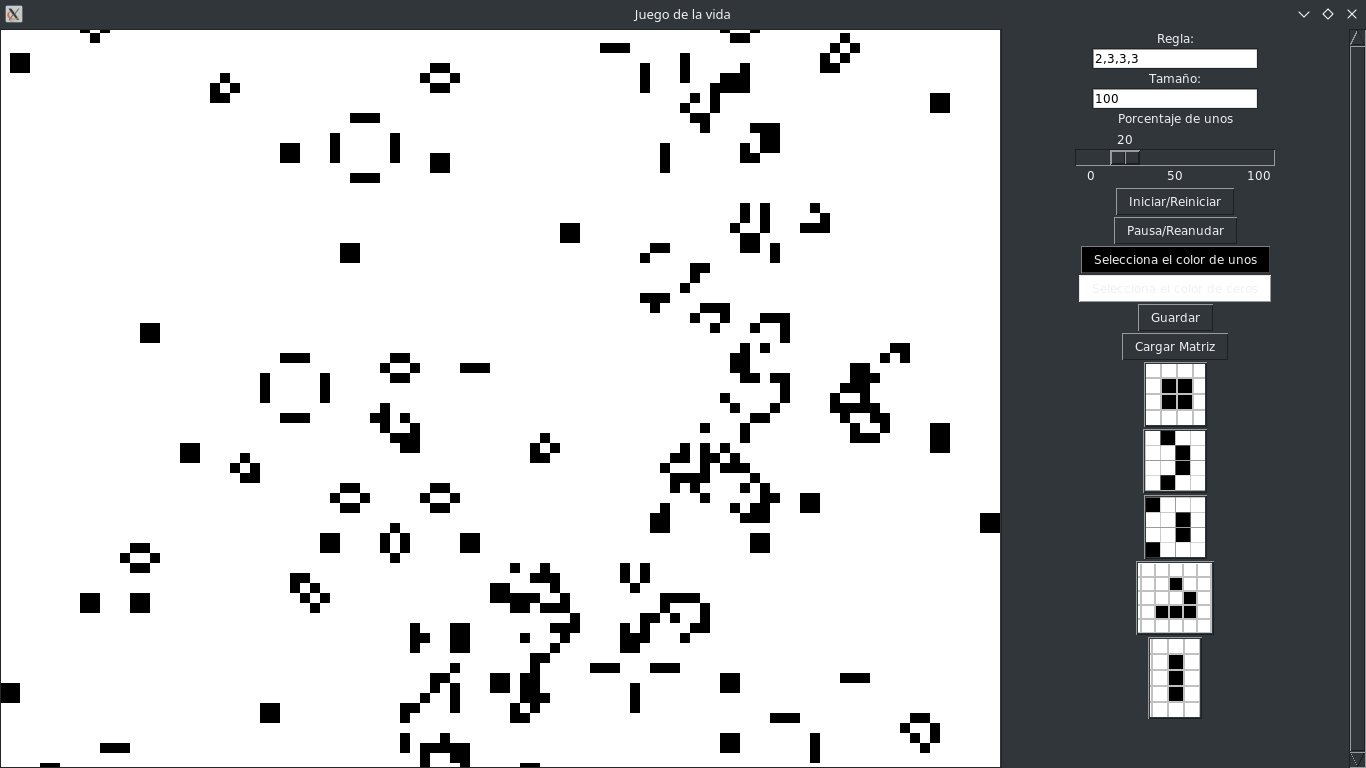
\includegraphics[width=12cm, height=8cm]{./img/life20.png}
 \caption{Regla de life con una probabilidad de unos de 20\%}
 \label{fig:life20}
\end{center}
\end{figure}

\begin{figure}[H]
\begin{center}
 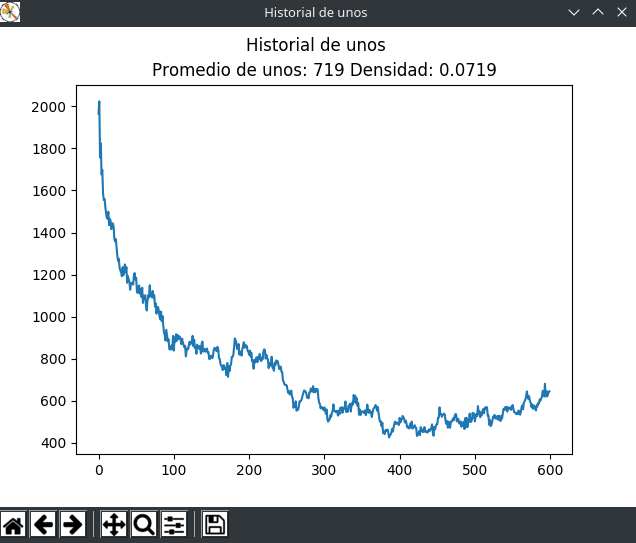
\includegraphics[width=12cm, height=8cm]{./img/life20grafica.png}
 \caption{Comportamiento de la población de la simulación anterior}
 \label{fig:life20grafica}
\end{center}
\end{figure}

\begin{figure}[H]
\begin{center}
 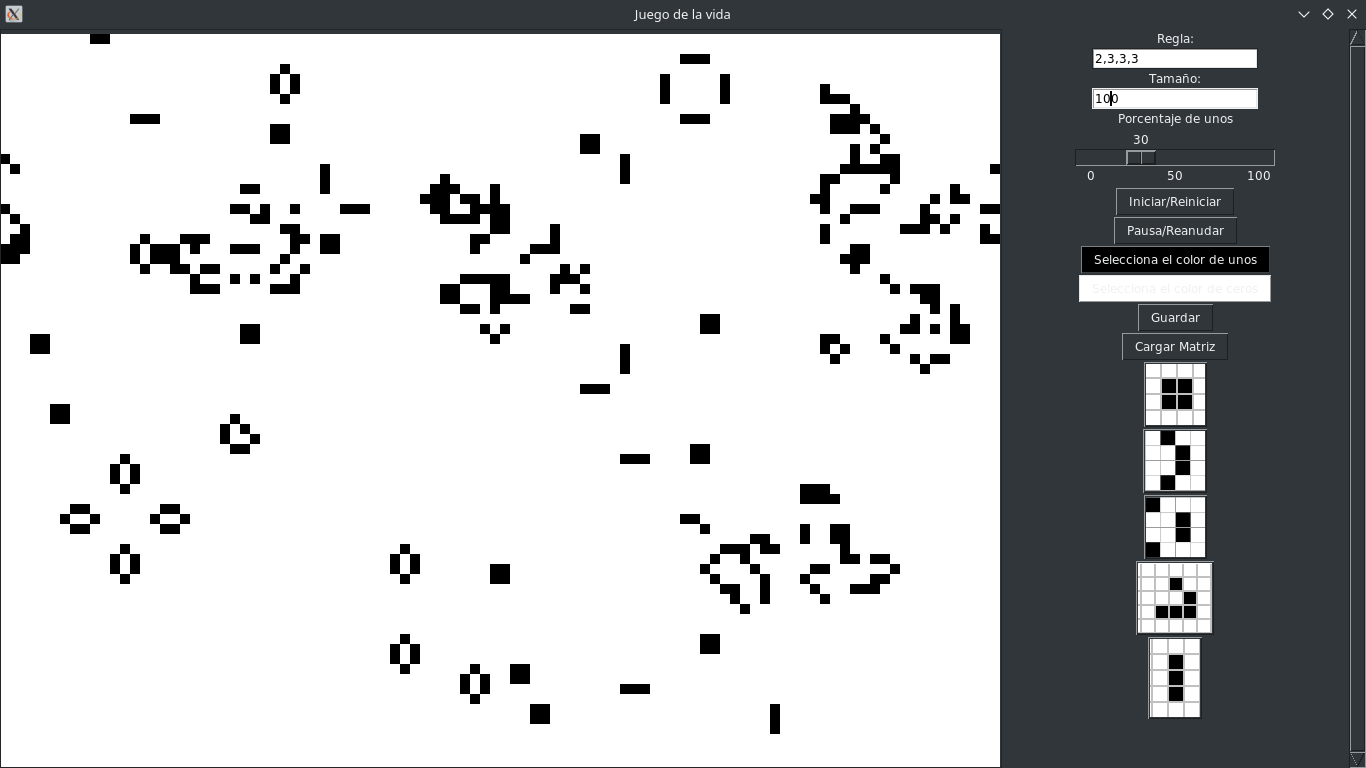
\includegraphics[width=12cm, height=8cm]{./img/life30.png}
 \caption{Regla de life con una probabilidad de unos de 30\%}
 \label{fig:life30}
\end{center}
\end{figure}

\begin{figure}[H]
\begin{center}
 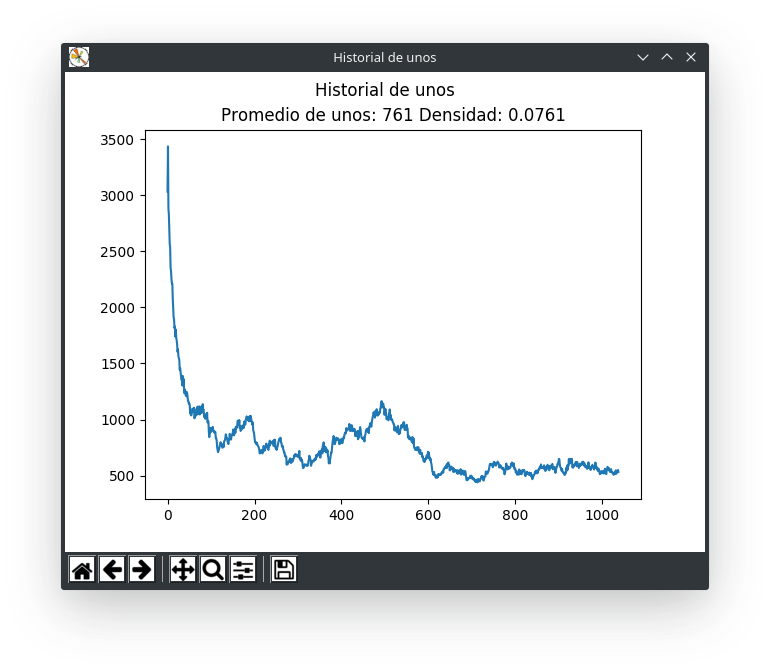
\includegraphics[width=12cm, height=8cm]{./img/life30grafica.png}
 \caption{Comportamiento de la población de la simulación anterior}
 \label{fig:life30grafica}
\end{center}
\end{figure}

\begin{figure}[H]
\begin{center}
 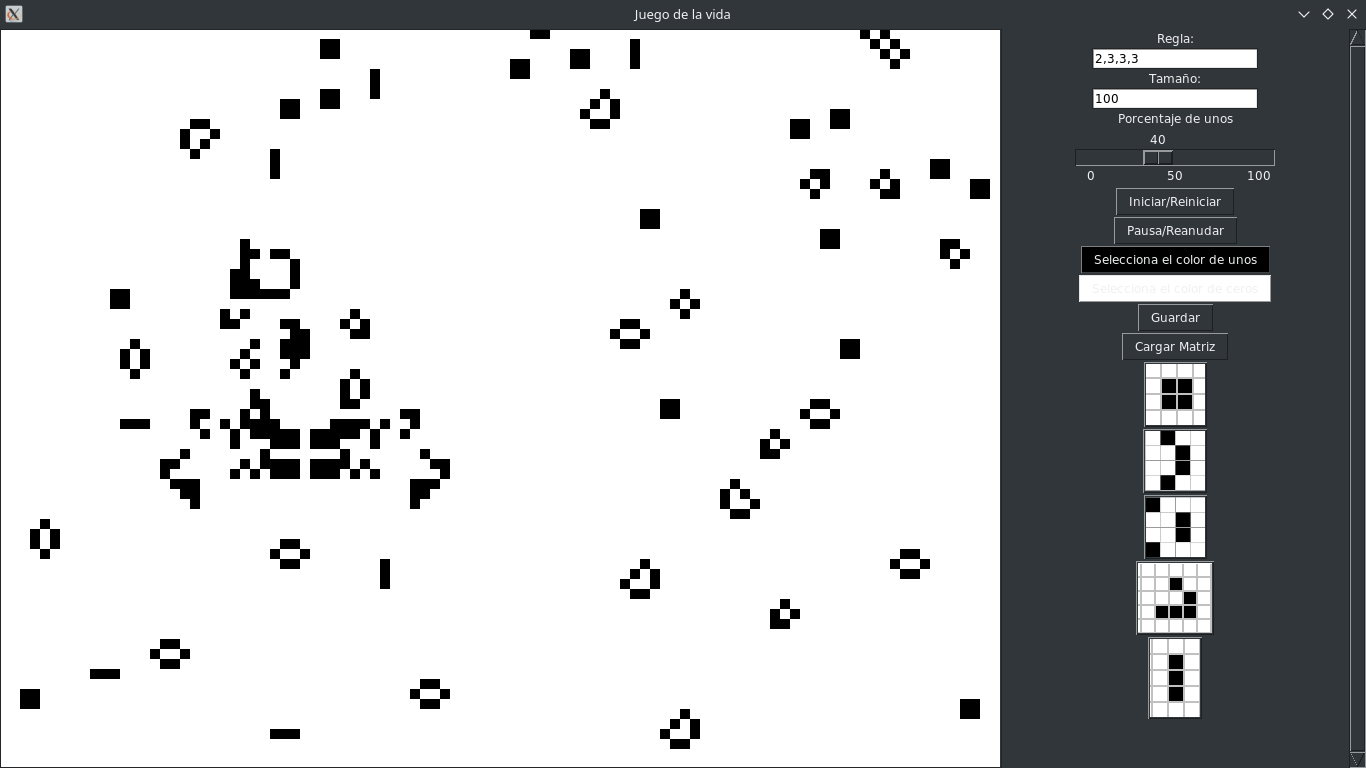
\includegraphics[width=12cm, height=8cm]{./img/life40.png}
 \caption{Regla de life con una probabilidad de unos de 40\%}
 \label{fig:life40}
\end{center}
\end{figure}

\begin{figure}[H]
\begin{center}
 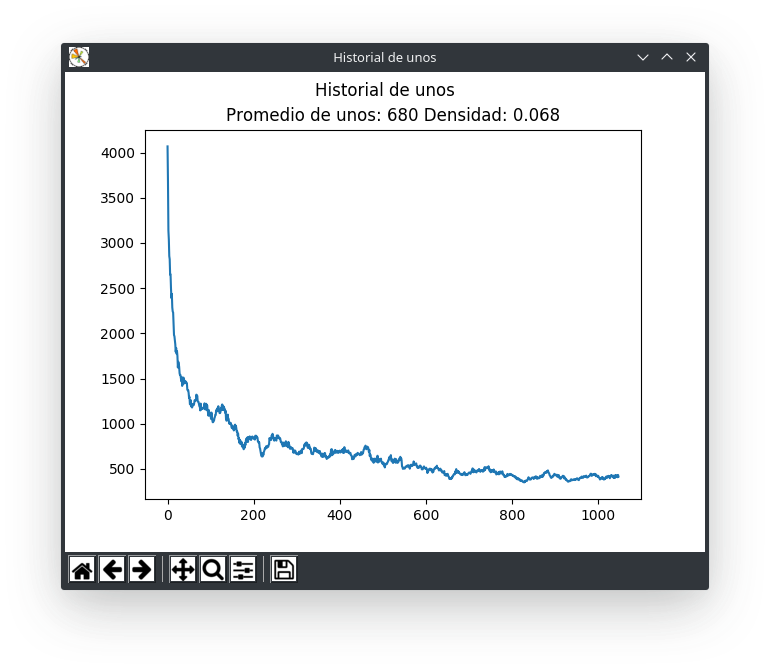
\includegraphics[width=12cm, height=8cm]{./img/life40grafica.png}
 \caption{Comportamiento de la población de la simulación anterior}
 \label{fig:life40grafica}
\end{center}
\end{figure}

\begin{figure}[H]
\begin{center}
 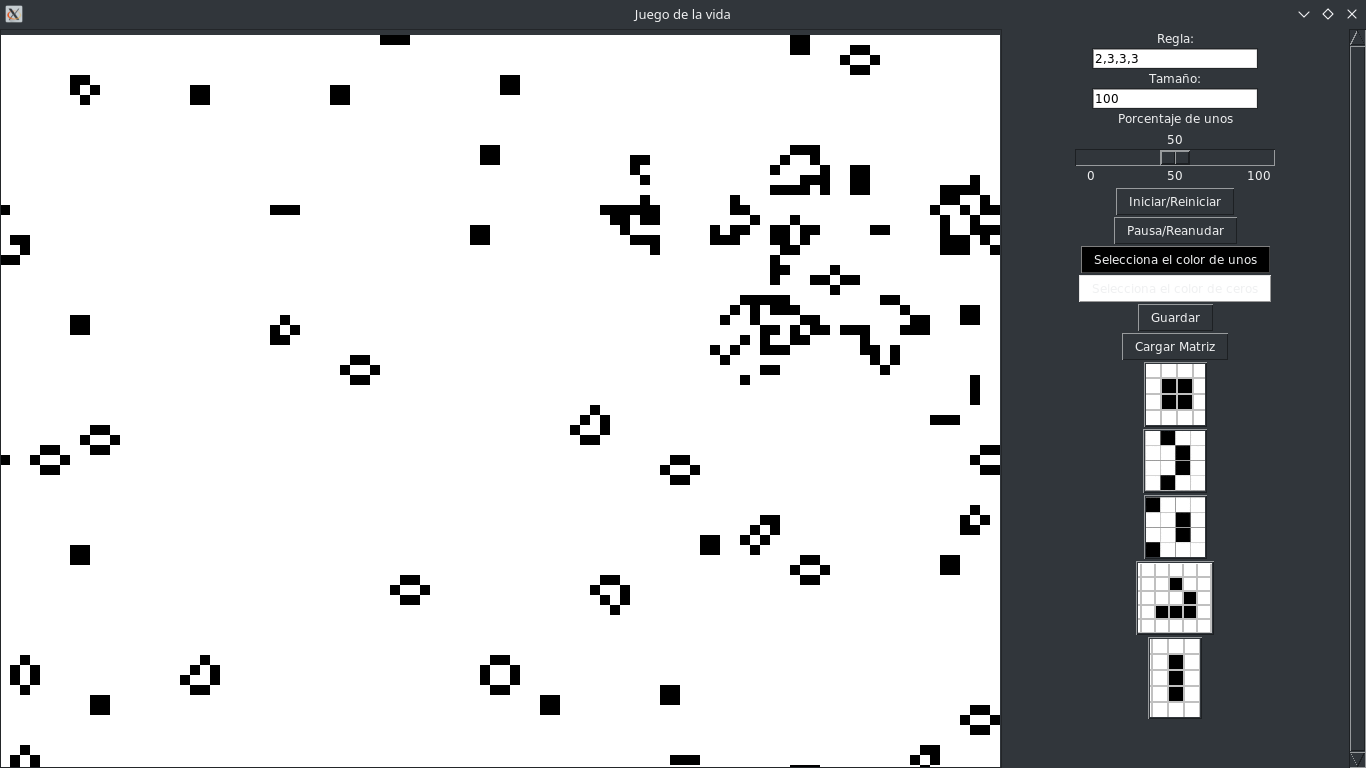
\includegraphics[width=12cm, height=8cm]{./img/life50.png}
 \caption{Regla de life con una probabilidad de unos de 50\%}
 \label{fig:life50}
\end{center}
\end{figure}

\begin{figure}[H]
\begin{center}
 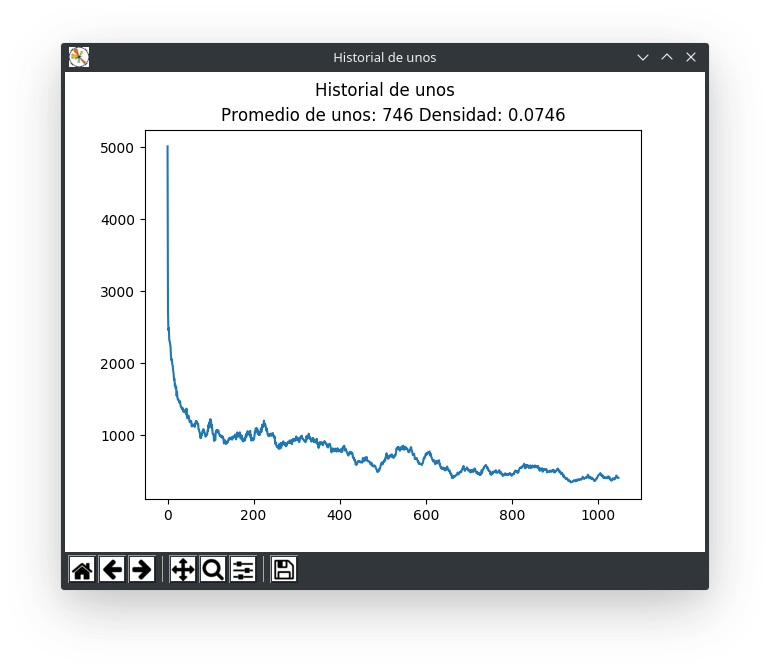
\includegraphics[width=12cm, height=8cm]{./img/life50grafica.png}
 \caption{Comportamiento de la población de la simulación anterior}
 \label{fig:life50grafica}
\end{center}
\end{figure}

\begin{figure}[H]
\begin{center}
 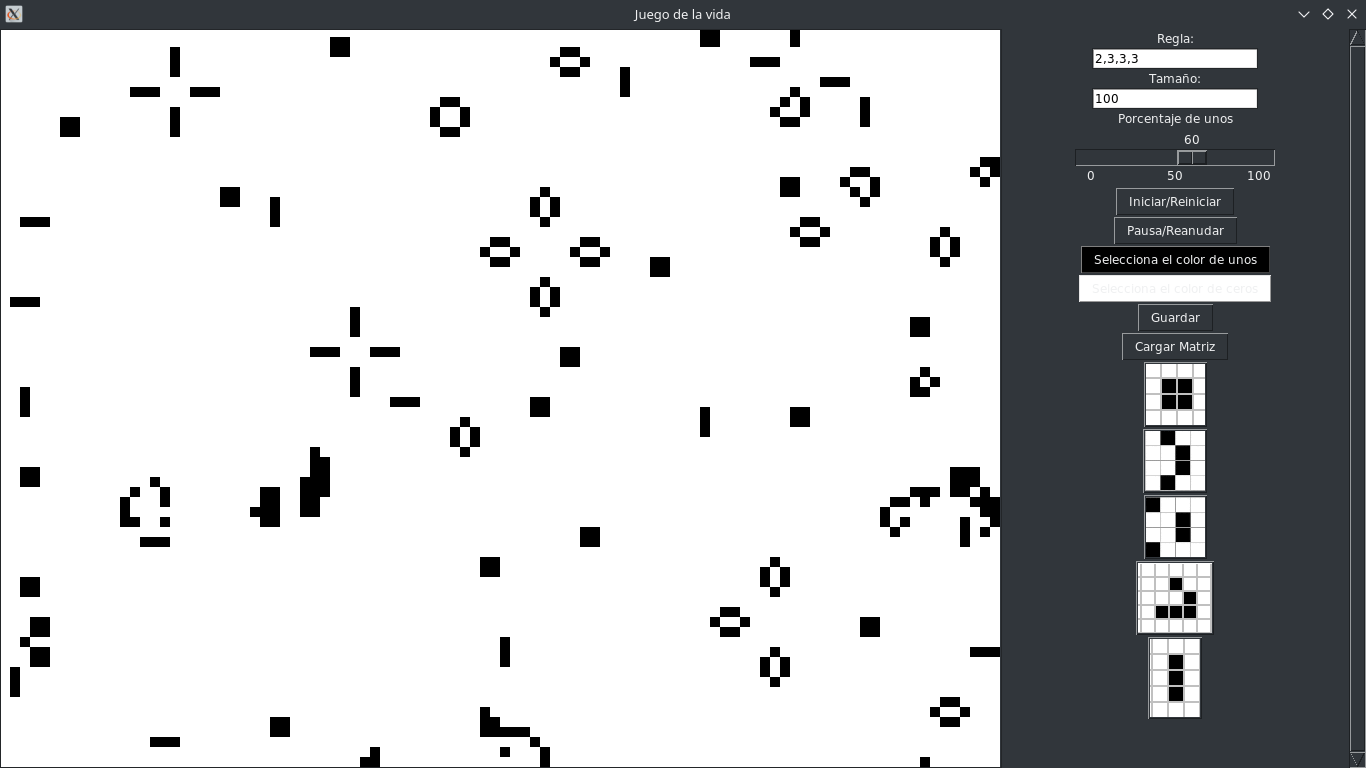
\includegraphics[width=12cm, height=8cm]{./img/life60.png}
 \caption{Regla de life con una probabilidad de unos de 60\%}
 \label{fig:life60}
\end{center}
\end{figure}

\begin{figure}[H]
\begin{center}
 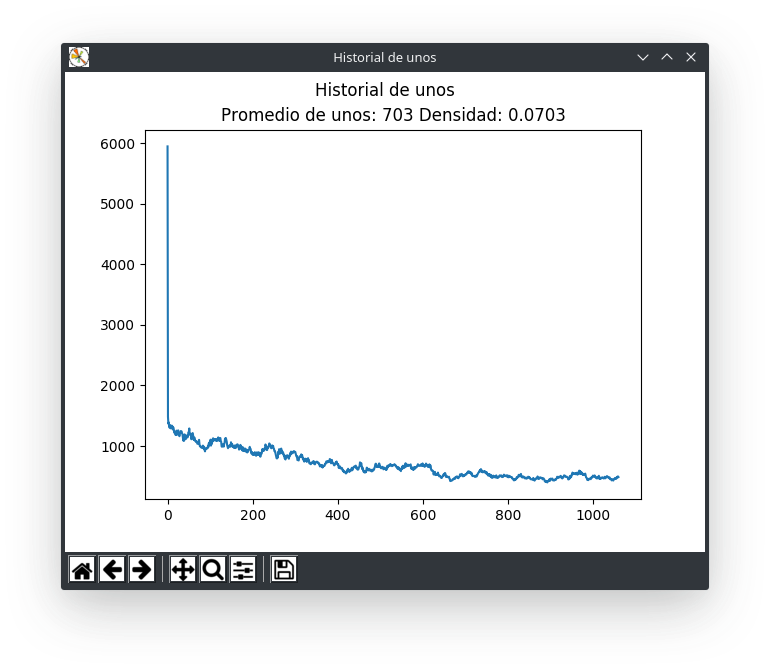
\includegraphics[width=12cm, height=8cm]{./img/life60grafica.png}
 \caption{Comportamiento de la población de la simulación anterior}
 \label{fig:life60grafica}
\end{center}
\end{figure}

\begin{figure}[H]
\begin{center}
 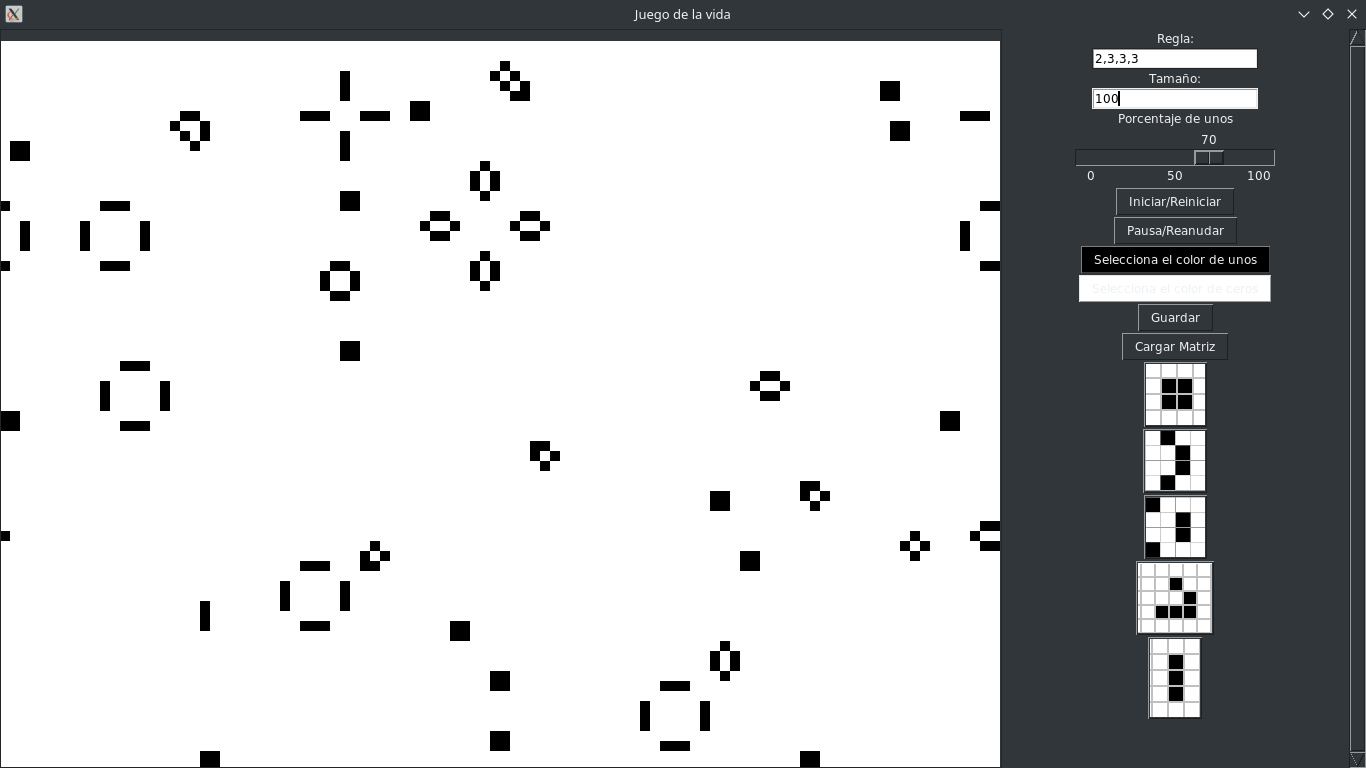
\includegraphics[width=12cm, height=8cm]{./img/life70.png}
 \caption{Regla de life con una probabilidad de unos de 70\%}
 \label{fig:life70}
\end{center}
\end{figure}

\begin{figure}[H]
\begin{center}
 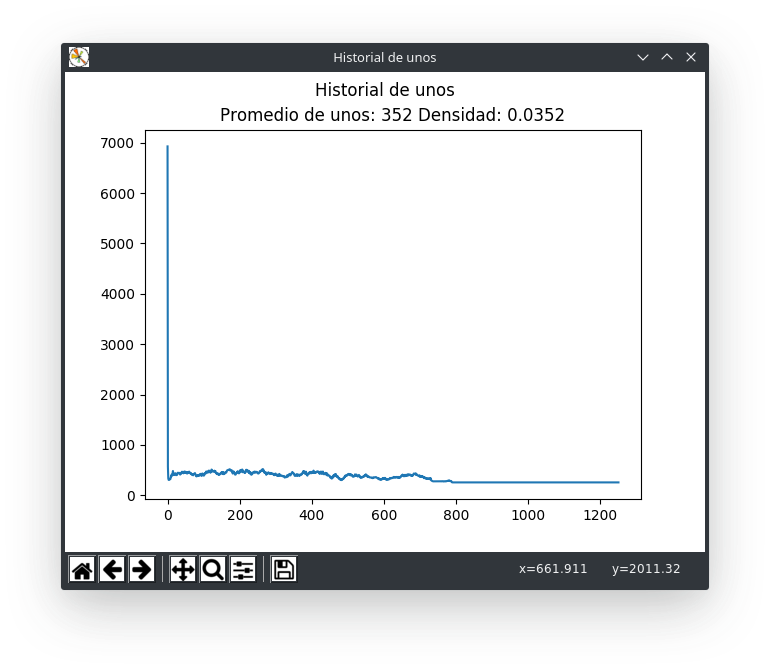
\includegraphics[width=12cm, height=8cm]{./img/life70grafica.png}
 \caption{Comportamiento de la población de la simulación anterior}
 \label{fig:life70grafica}
\end{center}
\end{figure}

\begin{figure}[H]
\begin{center}
 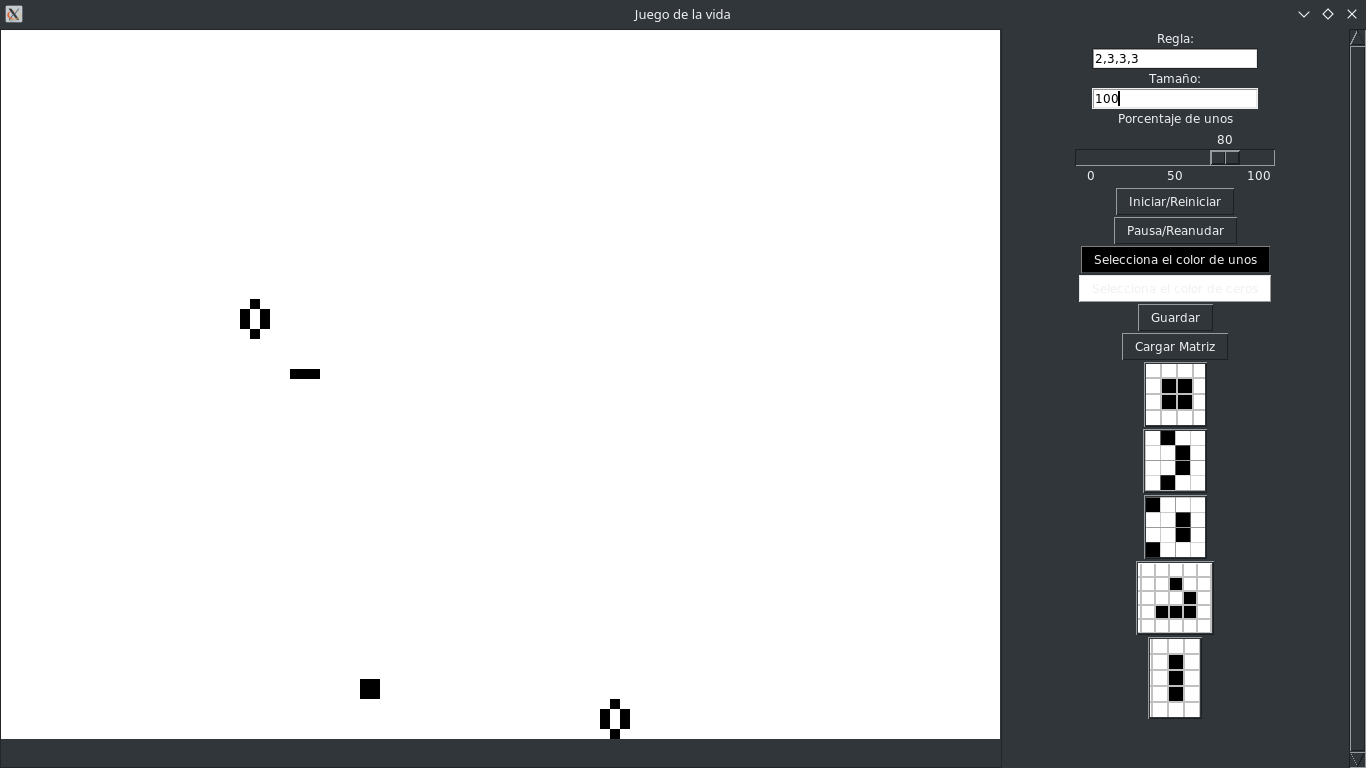
\includegraphics[width=12cm, height=8cm]{./img/life80.png}
 \caption{Regla de life con una probabilidad de unos de 80\%}
 \label{fig:life80}
\end{center}
\end{figure}

\begin{figure}[H]
\begin{center}
 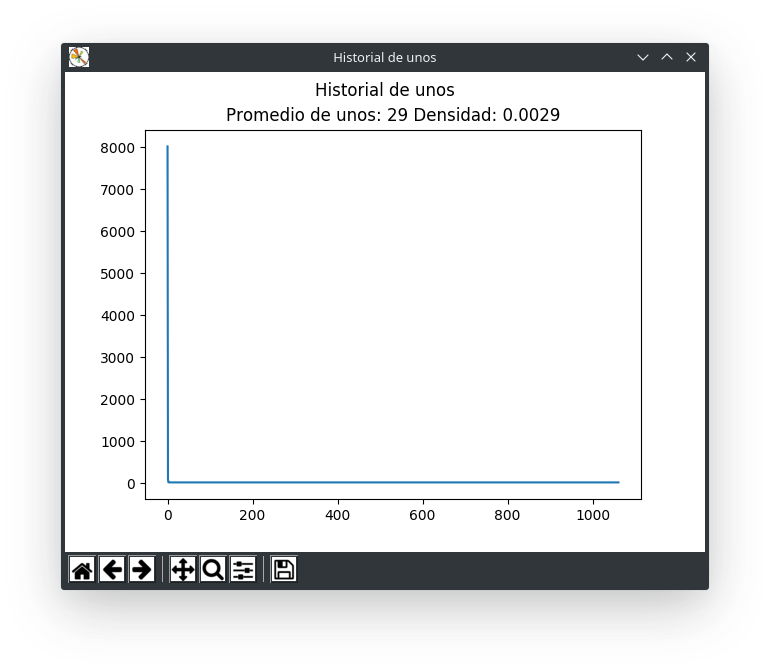
\includegraphics[width=12cm, height=8cm]{./img/life80grafica.png}
 \caption{Comportamiento de la población de la simulación anterior}
 \label{fig:life80grafica}
\end{center}
\end{figure}

\begin{figure}[H]
\begin{center}
 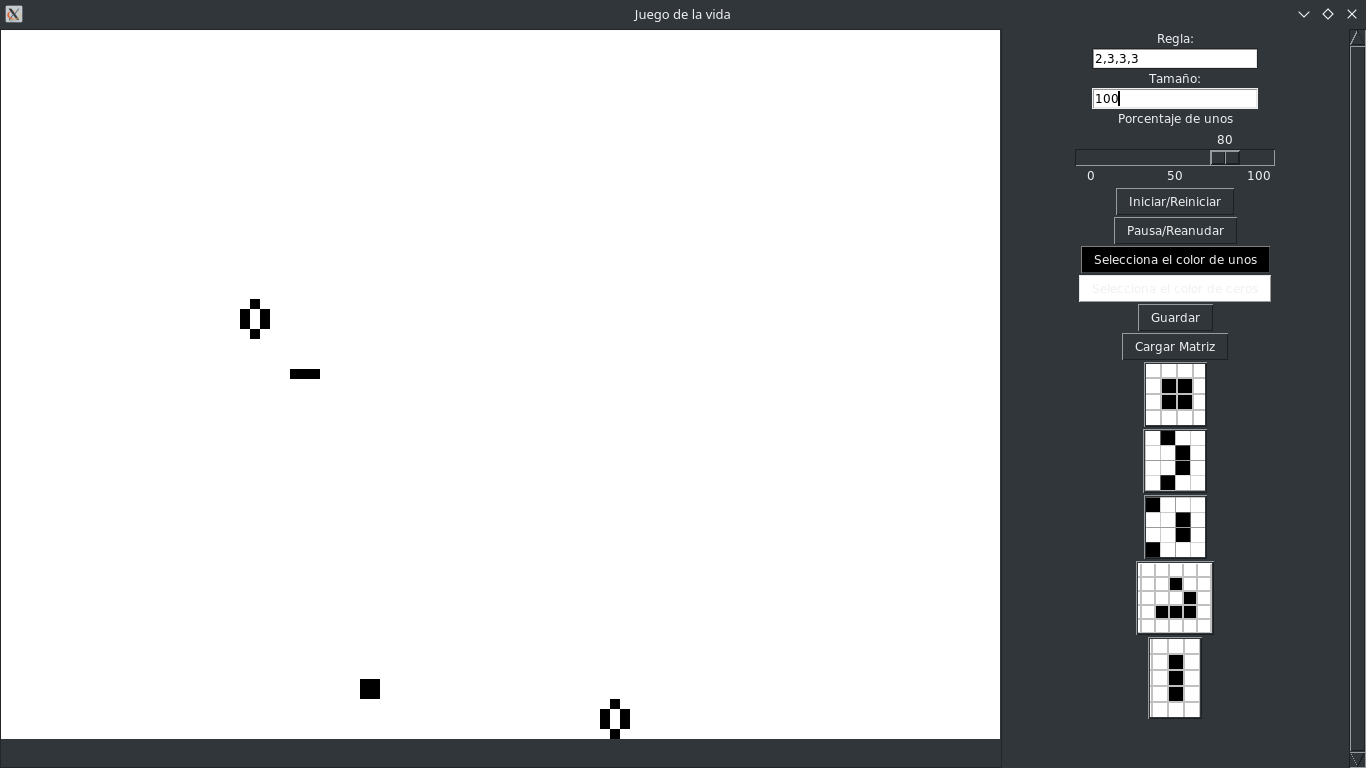
\includegraphics[width=12cm, height=8cm]{./img/life80.png}
 \caption{Regla de life con una probabilidad de unos de 90\%}
 \label{fig:life90}
\end{center}
\end{figure}

\begin{figure}[H]
\begin{center}
 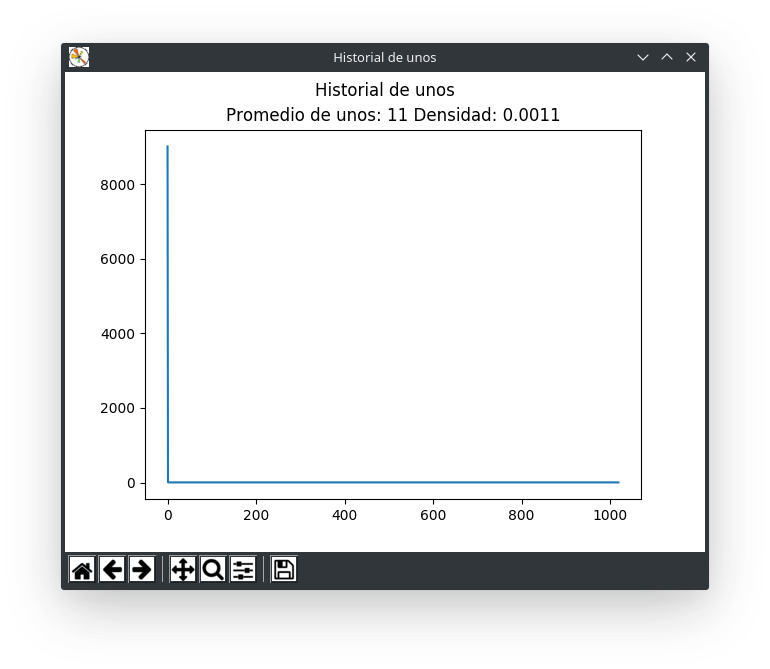
\includegraphics[width=12cm, height=8cm]{./img/life90grafica.png}
 \caption{Comportamiento de la población de la simulación anterior}
 \label{fig:life90grafica}
\end{center}
\end{figure}

\newpage
En todas las simulaciones se encuentra un comportamiento similar en el cual la población inicial es muy alta y de manera brusca disminuye y apartir de ahi decrece de manera lenta.

En la figura \ref{fig:life70} se aprecia asi que valor de densidad de la población tiende la regla de life, el valor es 0.0352, el resto de simulaciones tiende a un valor similar pero debido a que solo se trabajaron con 1000 generaciones no se logra apreciar por completo.

\newpage

\begin{figure}[H]
\begin{center}
 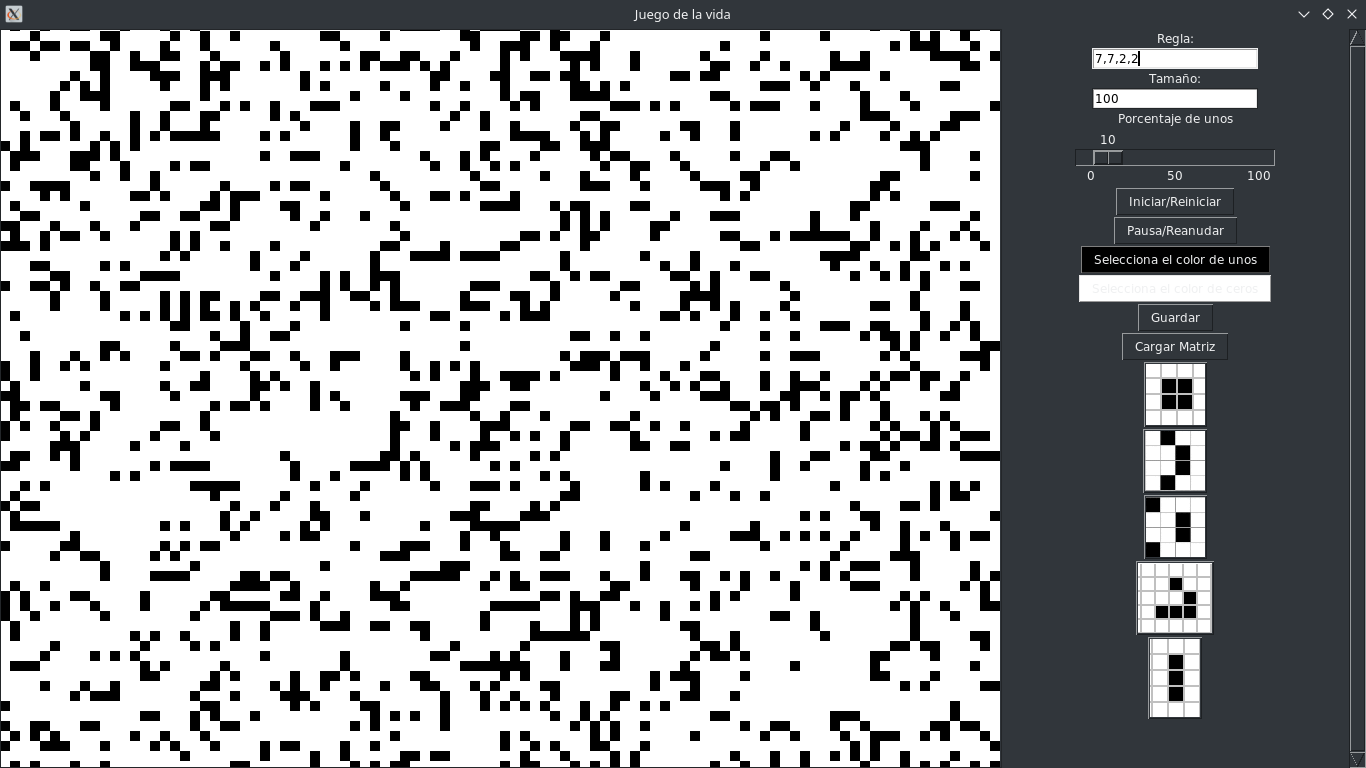
\includegraphics[width=12cm, height=8cm]{./img/diffusion10.png}
 \caption{Regla de difusión con una probabilidad de unos de 10\%}
 \label{fig:diffusion10}
\end{center}
\end{figure}

\begin{figure}[H]
\begin{center}
 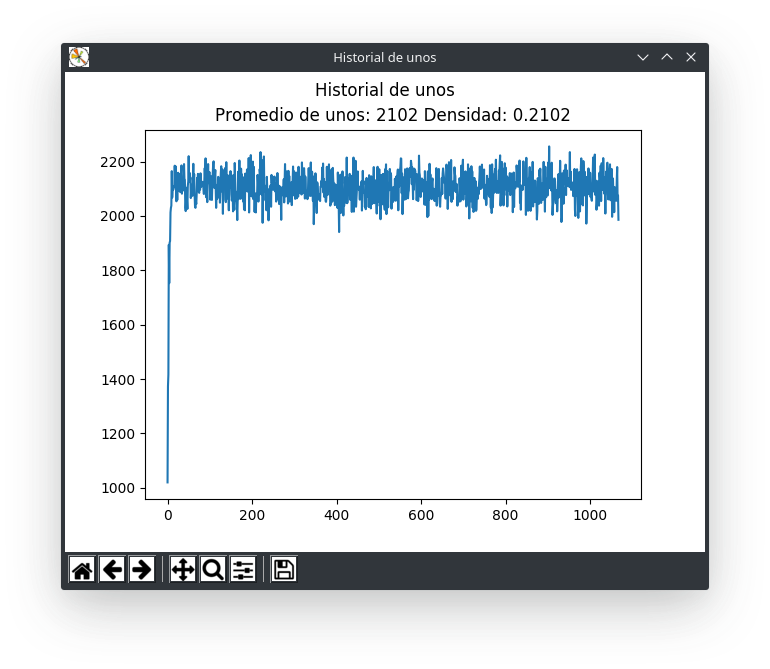
\includegraphics[width=12cm, height=8cm]{./img/diffusion10grafica.png}
 \caption{Comportamiento de la población de la simulación anterior}
 \label{fig:diffusion10grafica}
\end{center}
\end{figure}

\begin{figure}[H]
\begin{center}
 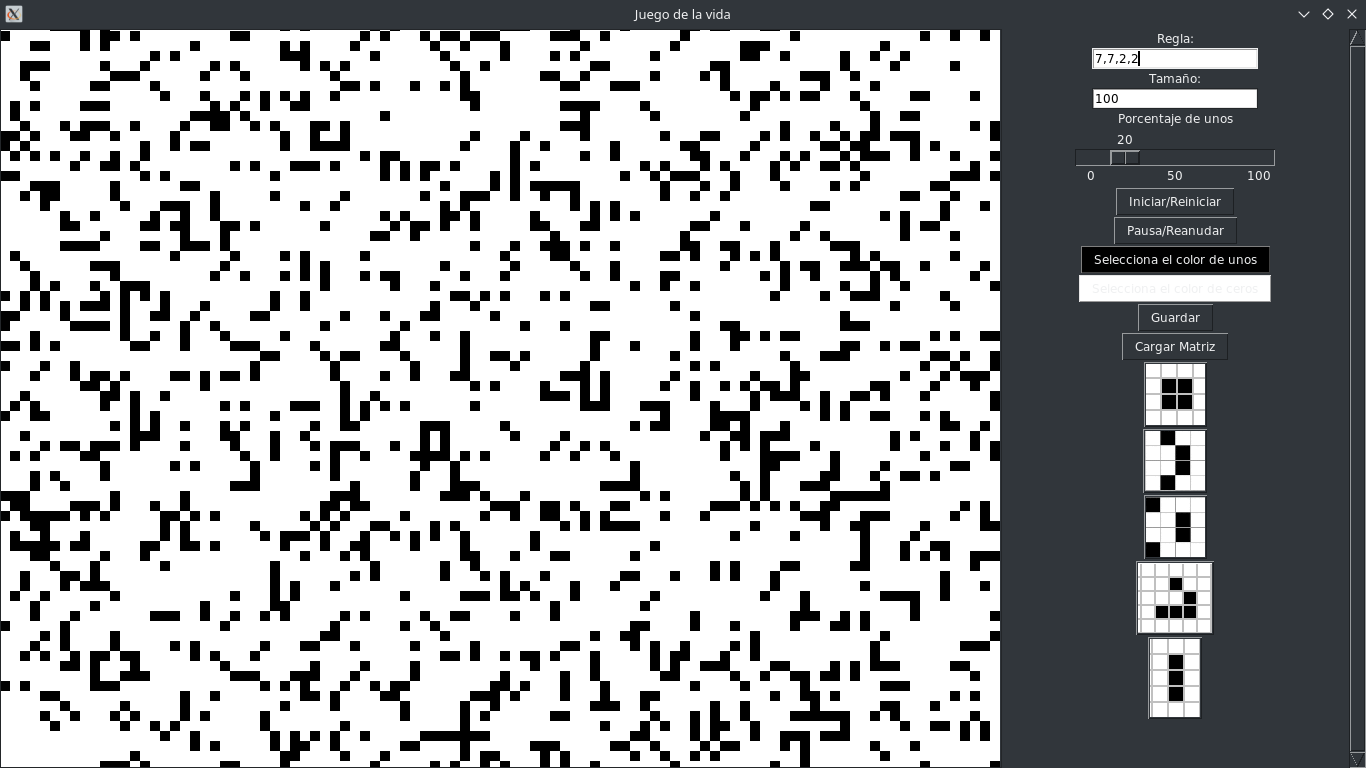
\includegraphics[width=12cm, height=8cm]{./img/diffusion20.png}
 \caption{Regla de difusión con una probabilidad de unos de 20\%}
 \label{fig:diffusion20}
\end{center}
\end{figure}

\begin{figure}[H]
\begin{center}
 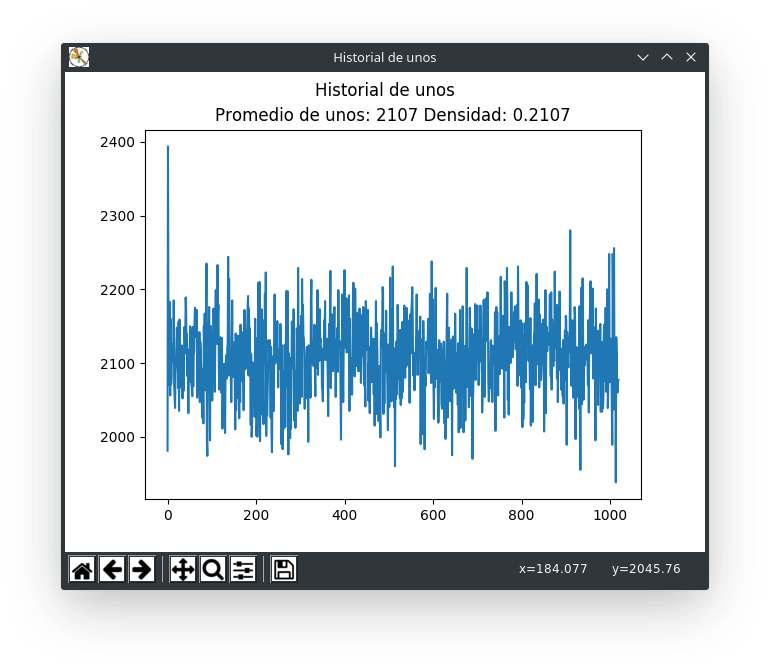
\includegraphics[width=12cm, height=8cm]{./img/diffusion20grafica.png}
 \caption{Comportamiento de la población de la simulación anterior}
 \label{fig:diffusion20grafica}
\end{center}
\end{figure}

\begin{figure}[H]
\begin{center}
 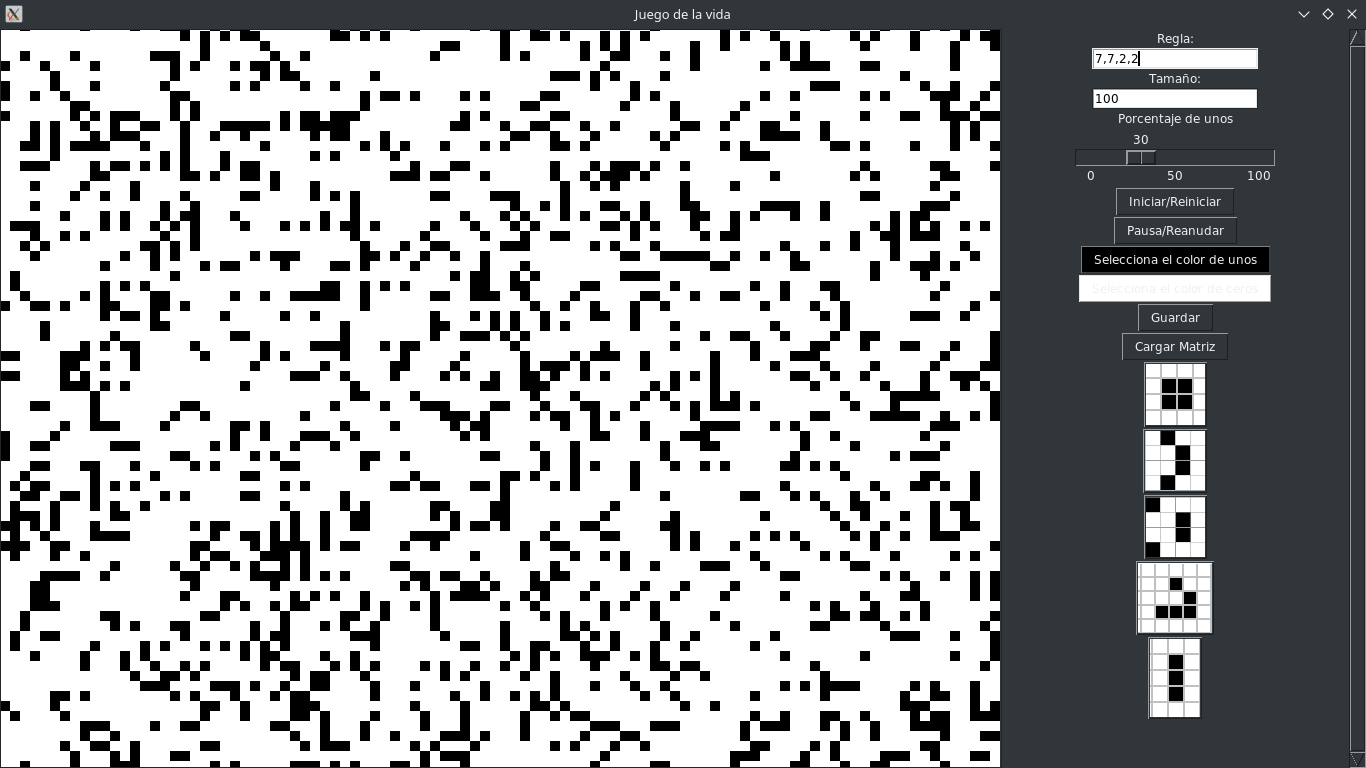
\includegraphics[width=12cm, height=8cm]{./img/diffusion30.png}
 \caption{Regla de difusión con una probabilidad de unos de 30\%}
 \label{fig:diffusion30}
\end{center}
\end{figure}

\begin{figure}[H]
\begin{center}
 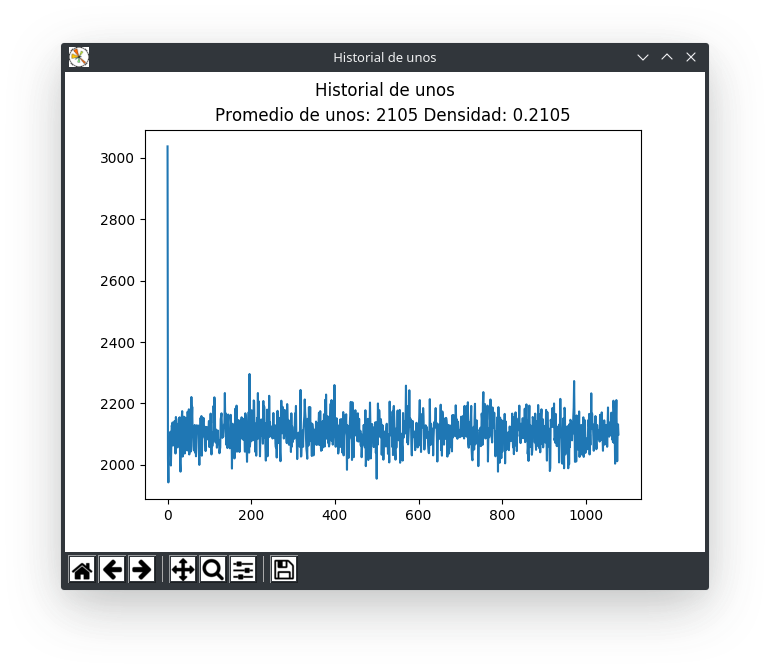
\includegraphics[width=12cm, height=8cm]{./img/diffusion30grafica.png}
 \caption{Comportamiento de la población de la simulación anterior}
 \label{fig:diffusion30grafica}
\end{center}
\end{figure}

\begin{figure}[H]
\begin{center}
 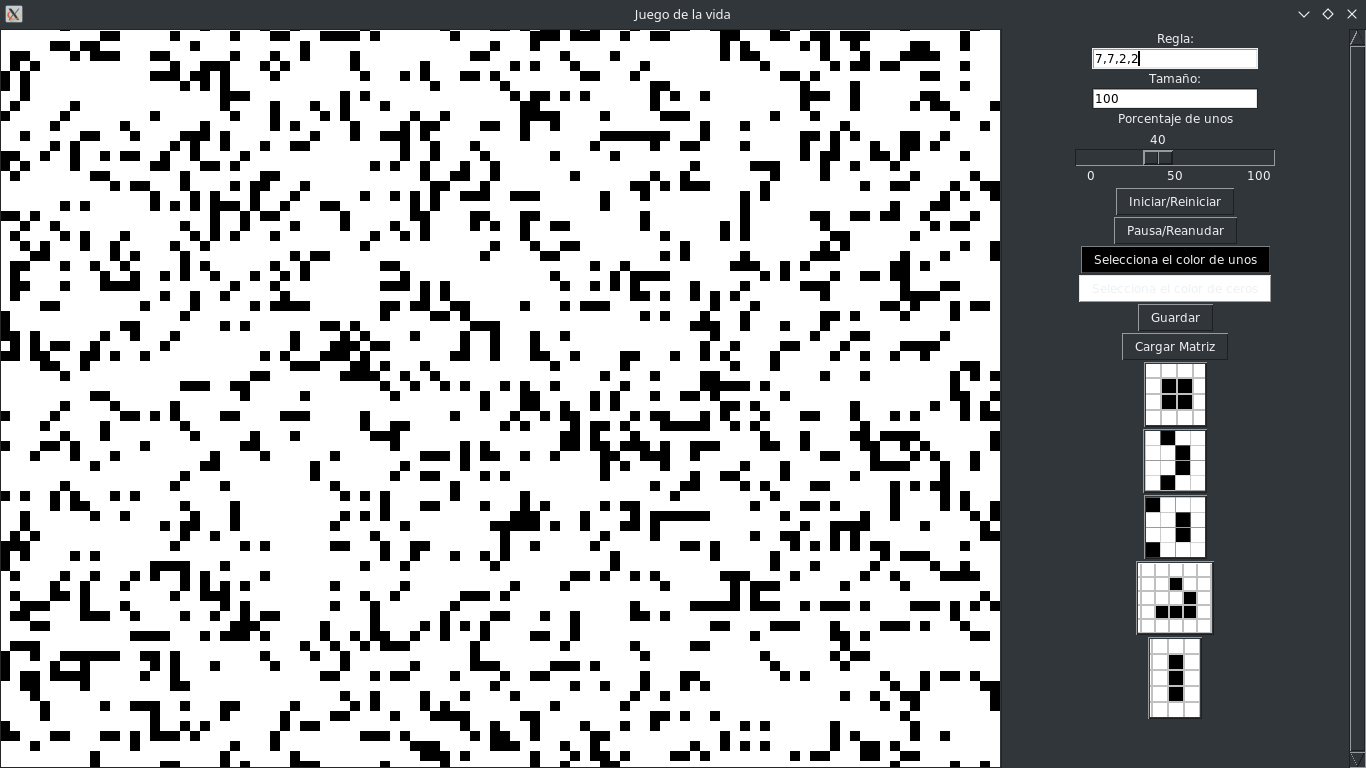
\includegraphics[width=12cm, height=8cm]{./img/diffusion40.png}
 \caption{Regla de difusión con una probabilidad de unos de 40\%}
 \label{fig:diffusion40}
\end{center}
\end{figure}

\begin{figure}[H]
\begin{center}
 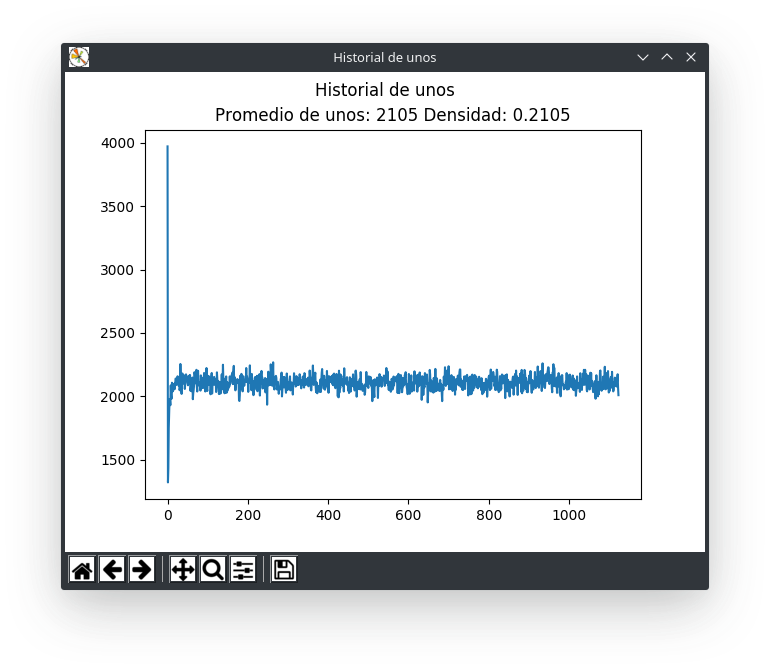
\includegraphics[width=12cm, height=8cm]{./img/diffusion40grafica.png}
 \caption{Comportamiento de la población de la simulación anterior}
 \label{fig:diffusion40grafica}
\end{center}
\end{figure}

\begin{figure}[H]
\begin{center}
 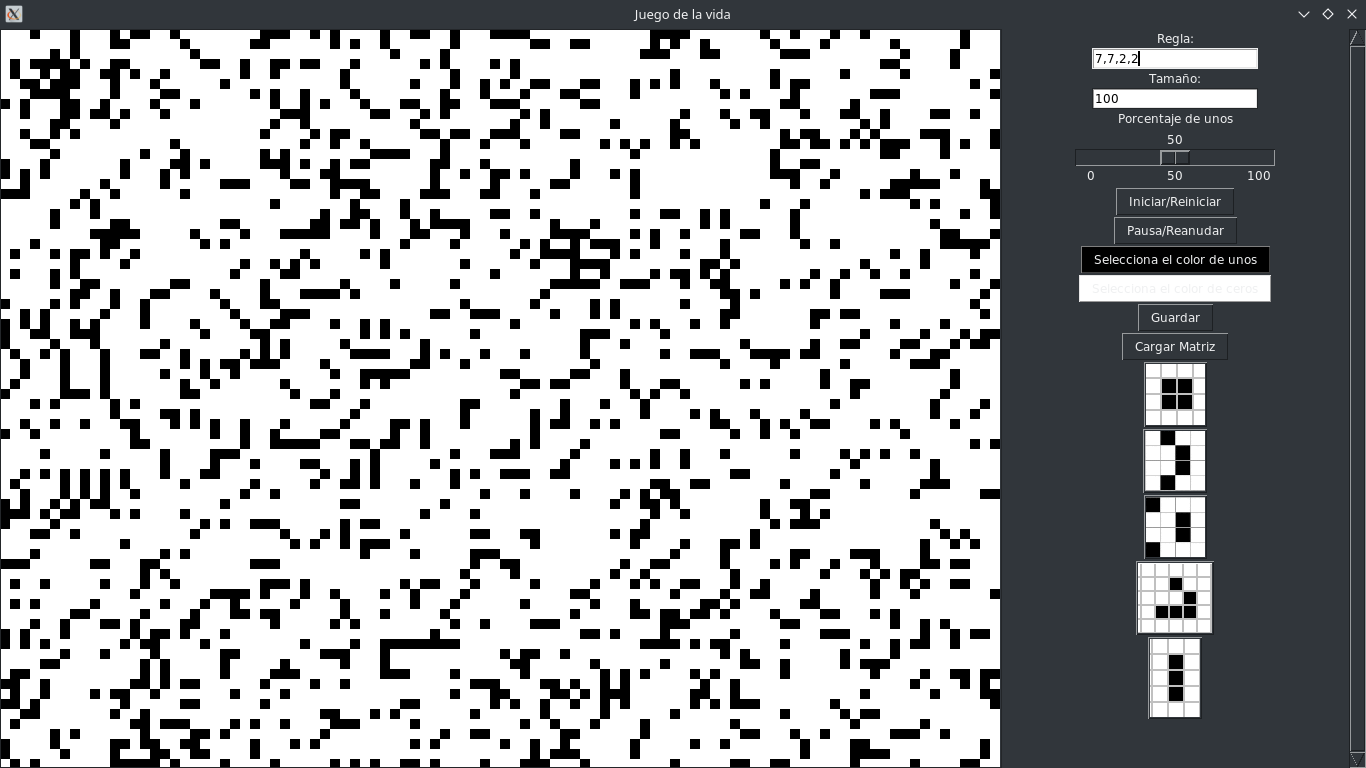
\includegraphics[width=12cm, height=8cm]{./img/diffusion50.png}
 \caption{Regla de difusión con una probabilidad de unos de 50\%}
 \label{fig:diffusion50}
\end{center}
\end{figure}

\begin{figure}[H]
\begin{center}
 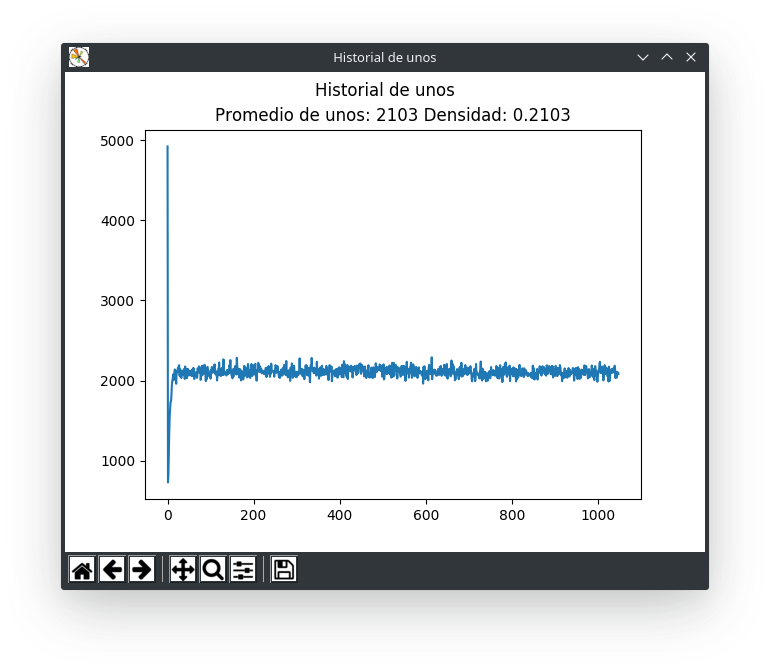
\includegraphics[width=12cm, height=8cm]{./img/diffusion50grafica.png}
 \caption{Comportamiento de la población de la simulación anterior}
 \label{fig:diffusion50grafica}
\end{center}
\end{figure}

\begin{figure}[H]
\begin{center}
 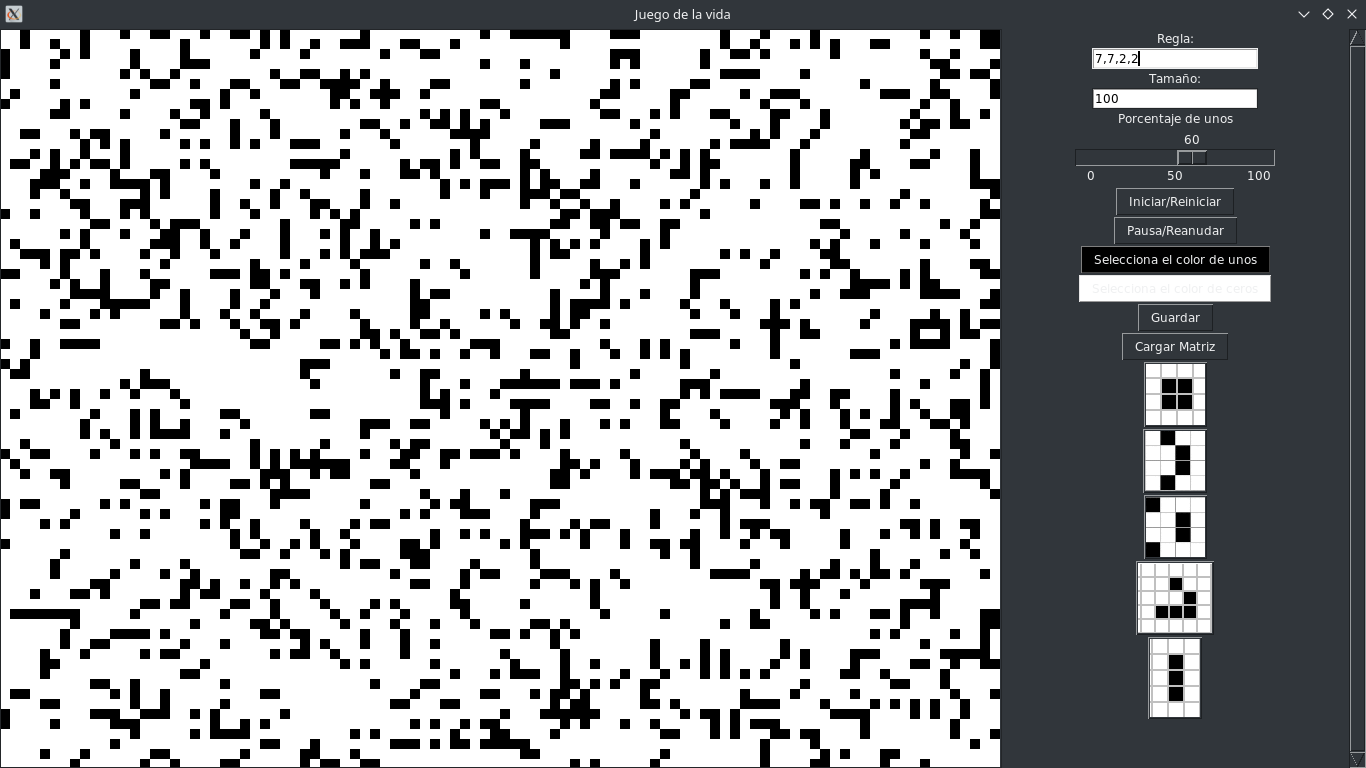
\includegraphics[width=12cm, height=8cm]{./img/diffusion60.png}
 \caption{Regla de difusión con una probabilidad de unos de 60\%}
 \label{fig:diffusion60}
\end{center}
\end{figure}

\begin{figure}[H]
\begin{center}
 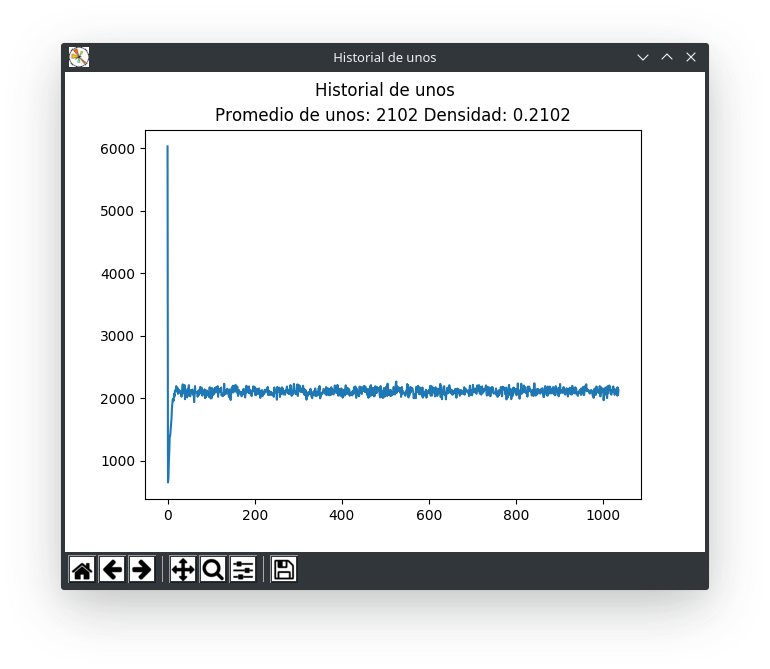
\includegraphics[width=12cm, height=8cm]{./img/diffusion60grafica.png}
 \caption{Comportamiento de la población de la simulación anterior}
 \label{fig:diffusion60grafica}
\end{center}
\end{figure}

\begin{figure}[H]
\begin{center}
 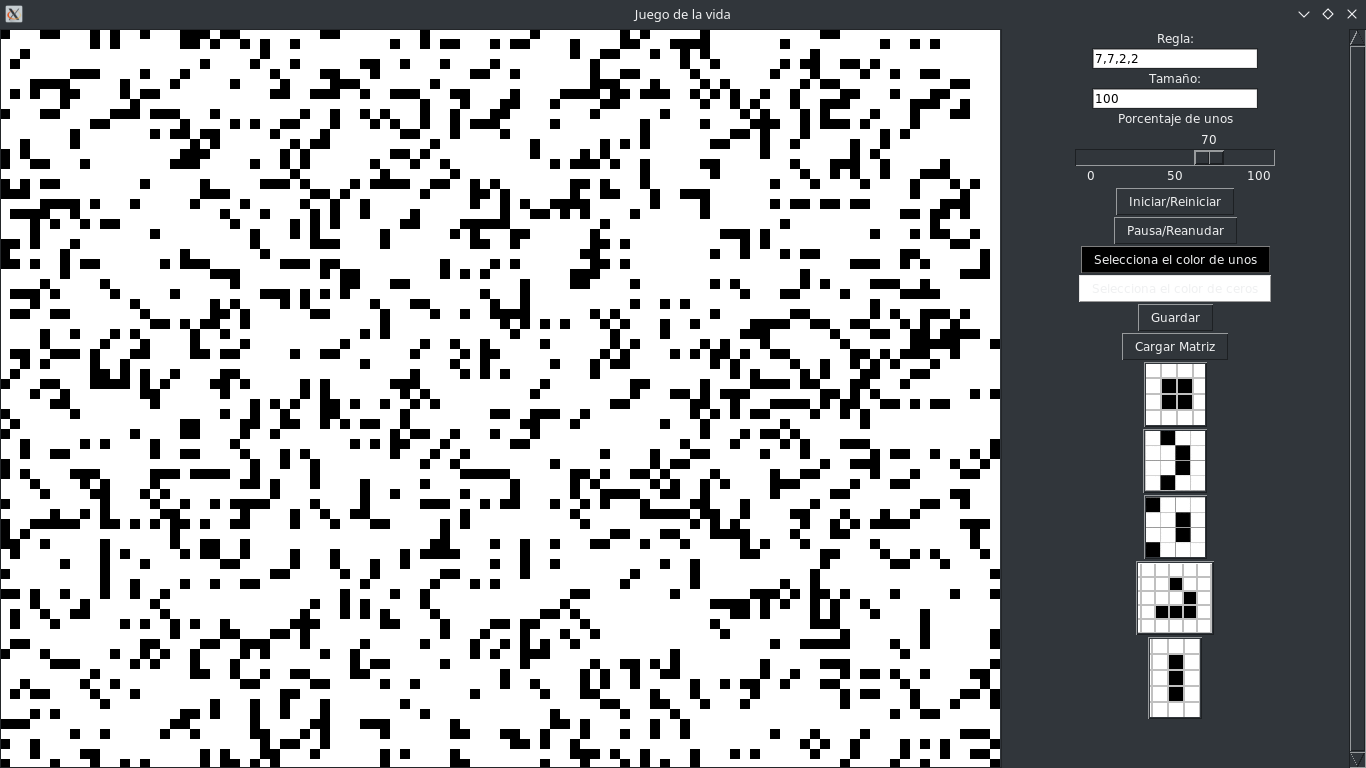
\includegraphics[width=12cm, height=8cm]{./img/diffusion70.png}
 \caption{Regla de difusión con una probabilidad de unos de 70\%}
 \label{fig:diffusion70}
\end{center}
\end{figure}

\begin{figure}[H]
\begin{center}
 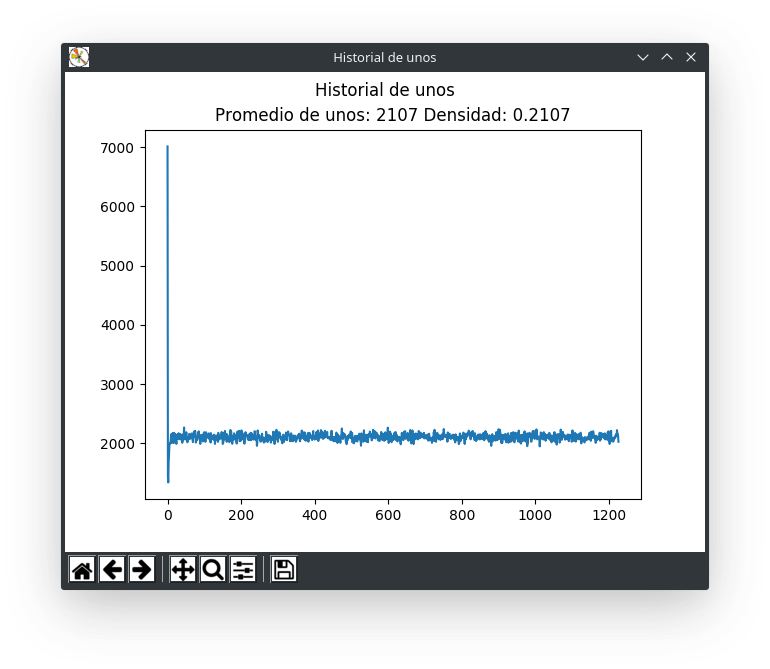
\includegraphics[width=12cm, height=8cm]{./img/diffusion70grafica.png}
 \caption{Comportamiento de la población de la simulación anterior}
 \label{fig:diffusion70grafica}
\end{center}
\end{figure}

\begin{figure}[H]
\begin{center}
 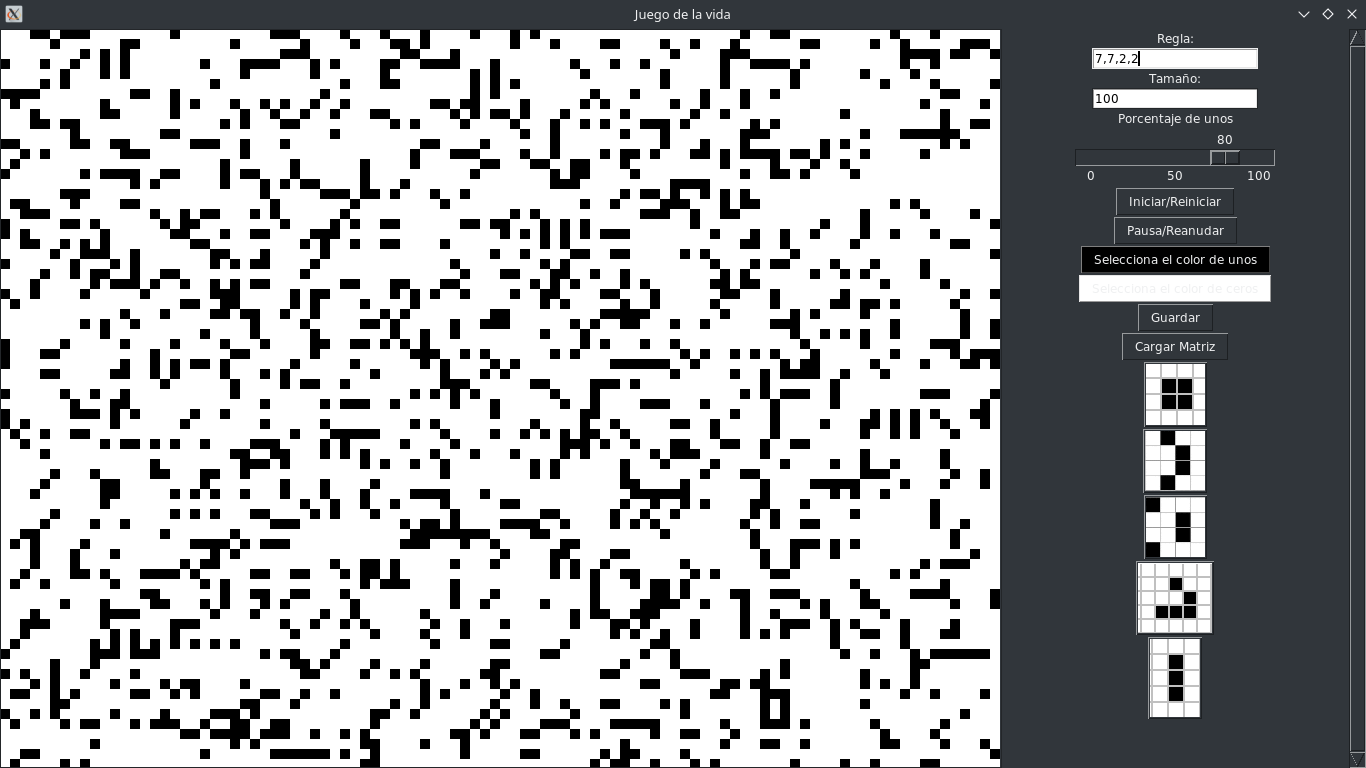
\includegraphics[width=12cm, height=8cm]{./img/diffusion80.png}
 \caption{Regla de difusión con una probabilidad de unos de 80\%}
 \label{fig:diffusion80}
\end{center}
\end{figure}

\begin{figure}[H]
\begin{center}
 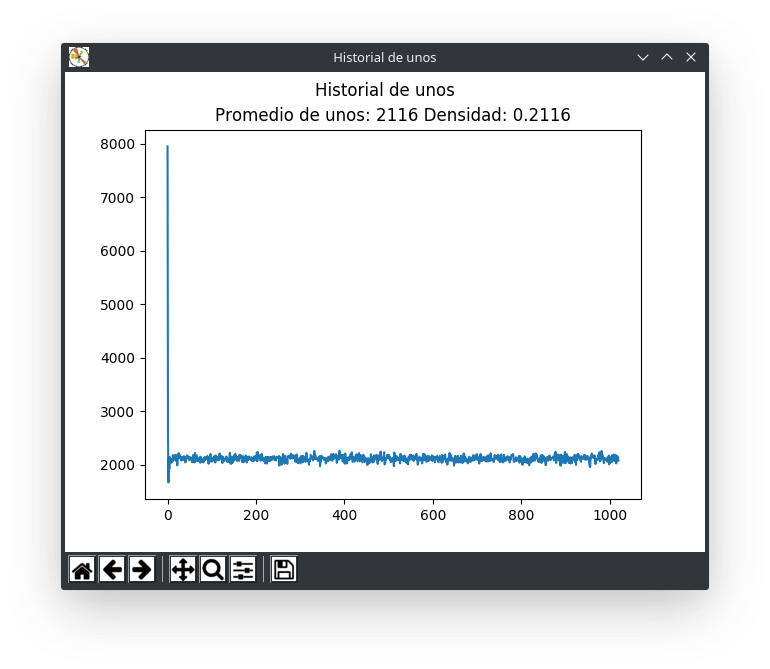
\includegraphics[width=12cm, height=8cm]{./img/diffusion80grafica.png}
 \caption{Comportamiento de la población de la simulación anterior}
 \label{fig:diffusion80grafica}
\end{center}
\end{figure}

\begin{figure}[H]
\begin{center}
 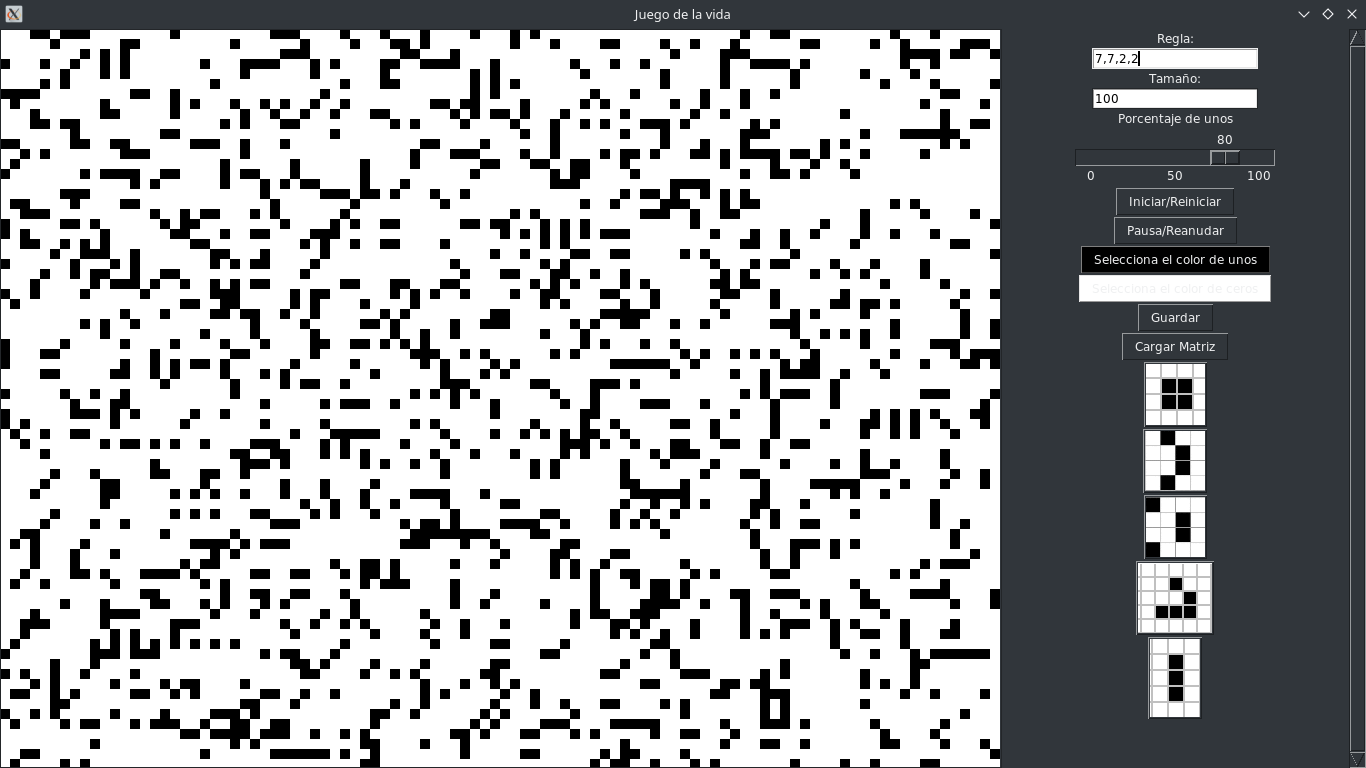
\includegraphics[width=12cm, height=8cm]{./img/diffusion80.png}
 \caption{Regla de difusión con una probabilidad de unos de 90\%}
 \label{fig:diffusion90}
\end{center}
\end{figure}

\begin{figure}[H]
\begin{center}
 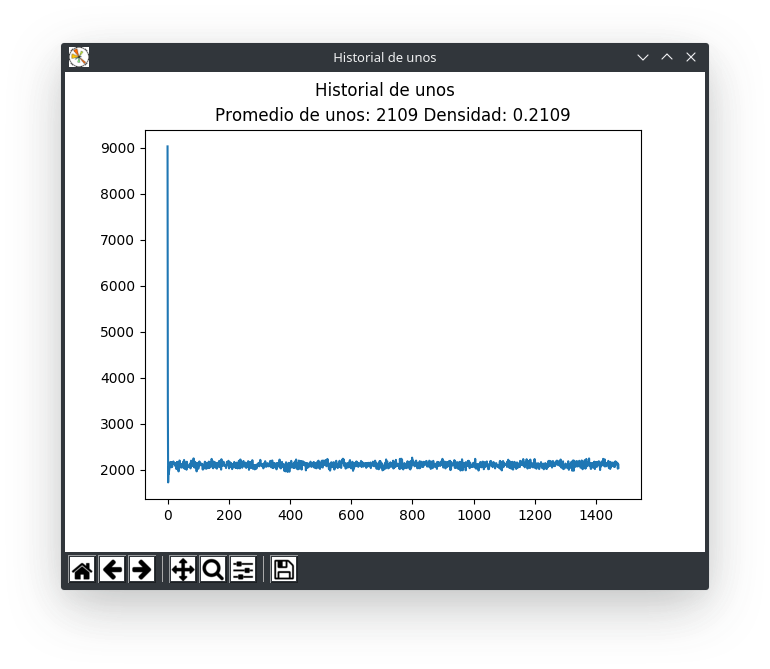
\includegraphics[width=12cm, height=8cm]{./img/diffusion90grafica.png}
 \caption{Comportamiento de la población de la simulación anterior}
 \label{fig:diffusion90grafica}
\end{center}
\end{figure}

Para la regla de difusión se podria decir que el comportamiento de la población es más estable que la de life debido a que en todas las simulaciones se llego a la densidad de población de 0.21 y el comportamiento de la gráfica es igual en todas las probabilidades de uno que se probaron en donde la población oscila entre un limite mayor y uno menor cerca de los 2000 individuos vivos lo cual es un comportamiento interesante.

Las pruebas que se realizaron fueron insertar los mosaicos ya definidos y ver como se comportan con las reglas de vida y de difusión.

\subsubsection{Insertar mosaicos}
\begin{figure}[H]
\begin{center}
 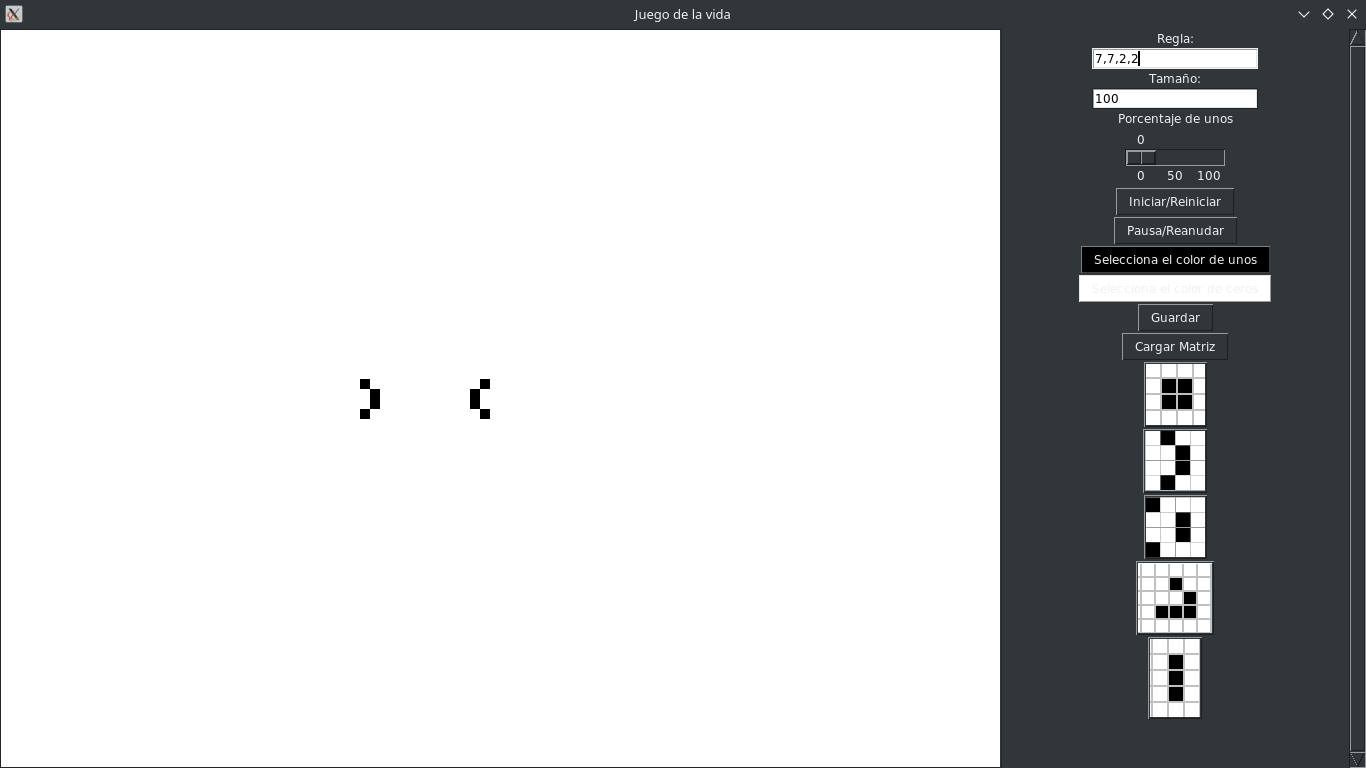
\includegraphics[width=12cm, height=8cm]{./img/inicio.png}
 \caption{Probando la regla 7722 con dos glider de frente}
 \label{fig:inicio}
\end{center}
\end{figure}

\begin{figure}[H]
\begin{center}
 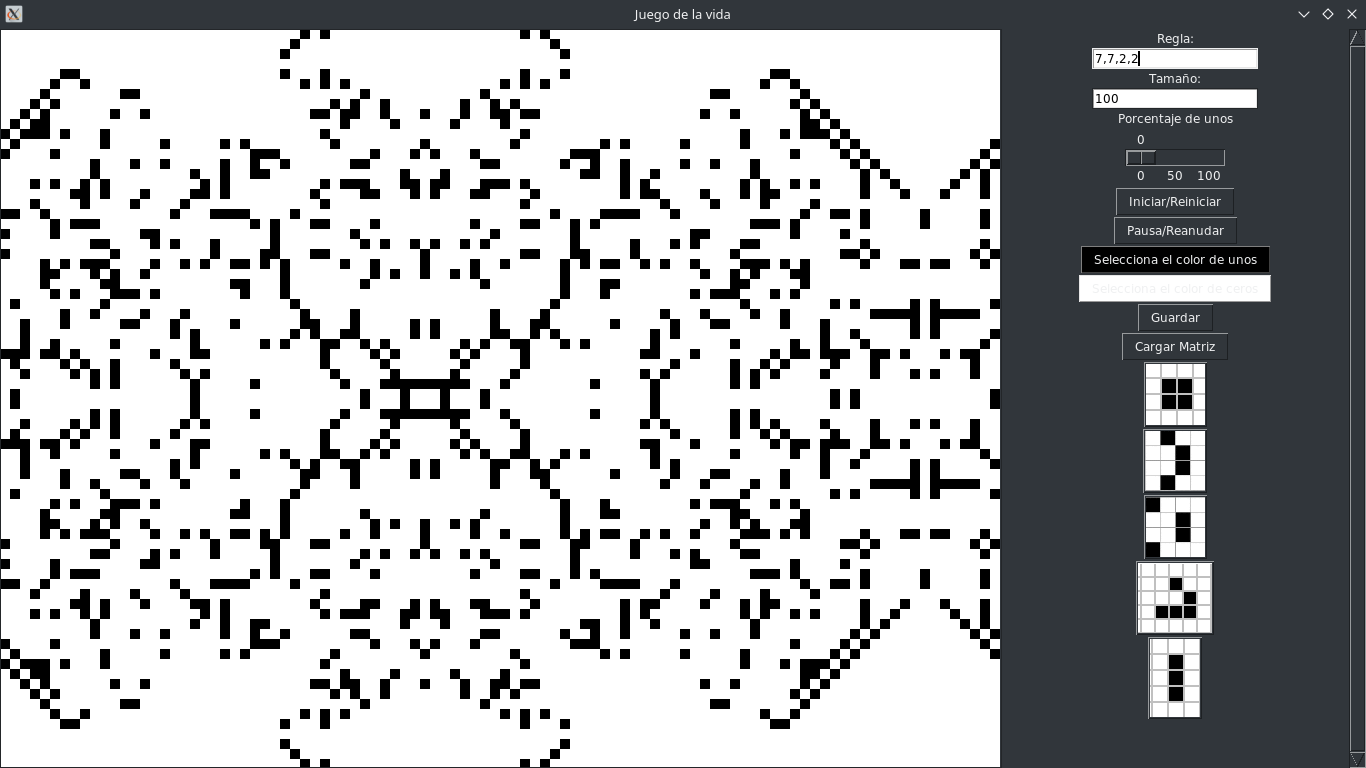
\includegraphics[width=12cm, height=8cm]{./img/final.png}
 \caption{Resultado producido por la configuración anterior}
 \label{fig:final}
\end{center}
\end{figure}


\begin{figure}[H]
\begin{center}
 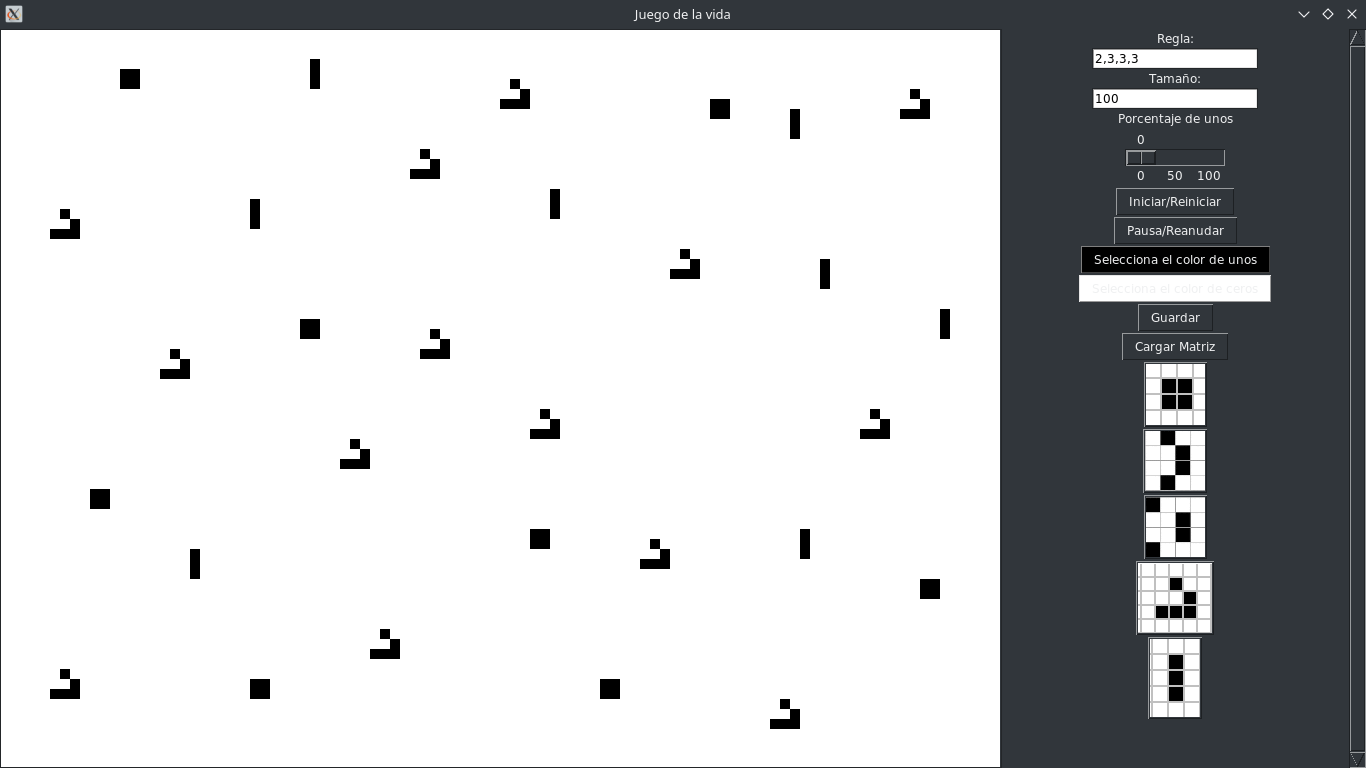
\includegraphics[width=12cm, height=8cm]{./img/prueba.png}
 \caption{Probando gliders, osciladores y patrones estáticos con la regla 2333}
 \label{fig:prueba}
\end{center}
\end{figure}

\begin{figure}[H]
\begin{center}
 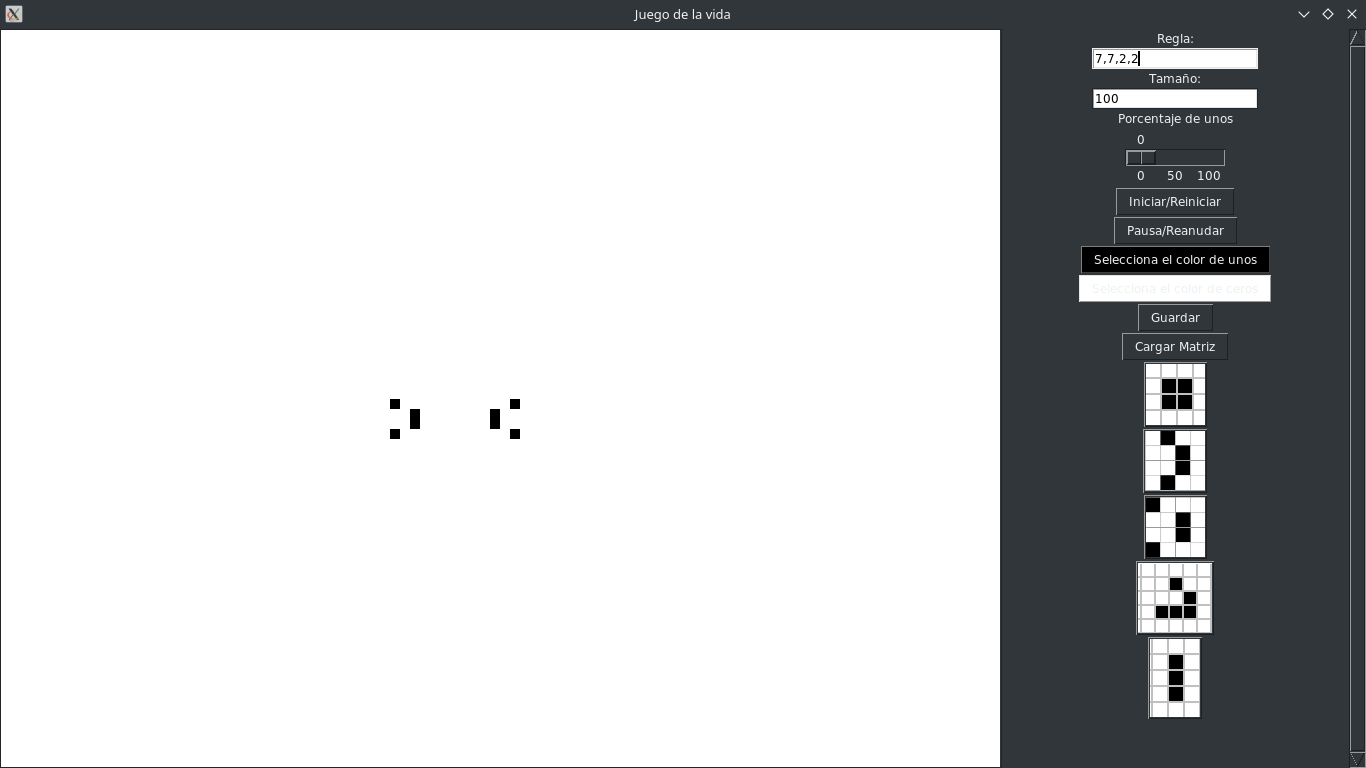
\includegraphics[width=12cm, height=8cm]{./img/inicio2.png}
 \caption{Probando la regla 7722 con dos glider de frente}
 \label{fig:inicio2}
\end{center}
\end{figure}

\begin{figure}[H]
\begin{center}
 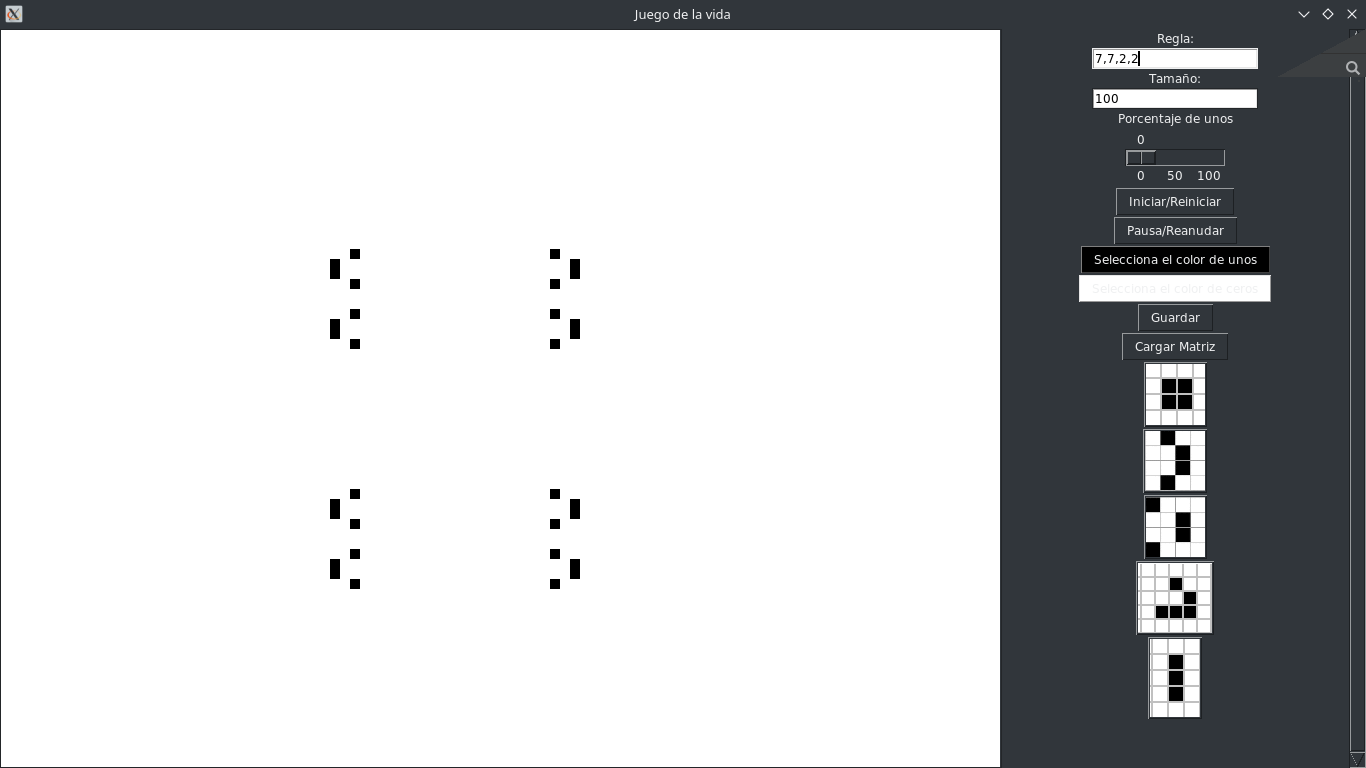
\includegraphics[width=12cm, height=8cm]{./img/final2.png}
 \caption{Resultado producido por la configuración anterior}
 \label{fig:final2}
\end{center}
\end{figure}

\subsection{Conclusiones}
Al hacer y probar este programa se pudieron solucionar dos cuestiones, la primera es si existe una configuración el la cual el numero de células no se termine, y la respuesta a esto es que exista un oscilador el cual cambia su posición a lo largo del tiempo, otra posible opción es que haya figuras como un bloque formado por 4 cuadros en el cual no hay cambios.

La siguiente cuestión es si existe una configuración en la cual la población crezca indefinidamente. Para lograr esto es indispensable tener un espacio que sea infinito en el cual se puedan propagar las células a través del tiempo, ya que si no se cuenta con esto en algún punto se tendrán tantos elementos vivos que empezaran a morir por sobre población.

Respecto a los patrones, los comportamientos que se generan al insertar distintos patrones en las dos reglas que tenemos resultan bastante interesante principalmente los gliders ya que estos son los que generan las figuras más complejas a partir de figuras tan simples y pequeñas y que con unas pocas generación crecen de una forma muy acelerada
